%%% Hlavní soubor. Zde se definují základní parametry a odkazuje se na ostatní části. %%%

%% Verze pro jednostranný tisk:
% Okraje: levý 40mm, pravý 25mm, horní a dolní 25mm
% (ale pozor, LaTeX si sám přidává 1in)
\documentclass[12pt,a4paper]{report}
\setlength\textwidth{145mm}
\setlength\textheight{247mm}
\setlength\oddsidemargin{15mm}
\setlength\evensidemargin{15mm}
\setlength\topmargin{0mm}
\setlength\headsep{0mm}
\setlength\headheight{0mm}
% \openright zařídí, aby následující text začínal na pravé straně knihy
\let\openright=\clearpage

%% Pokud tiskneme oboustranně:
% \documentclass[12pt,a4paper,twoside,openright]{report}
% \setlength\textwidth{145mm}
% \setlength\textheight{247mm}
% \setlength\oddsidemargin{14.2mm}
% \setlength\evensidemargin{0mm}
% \setlength\topmargin{0mm}
% \setlength\headsep{0mm}
% \setlength\headheight{0mm}
% \let\openright=\cleardoublepage

%% Vytváříme PDF/A-2u
\usepackage[a-2u]{pdfx}

%% Přepneme na českou sazbu a fonty Latin Modern
\usepackage[czech]{babel}
\usepackage{lmodern}
\usepackage[T1]{fontenc}
\usepackage{textcomp}

%% Použité kódování znaků: obvykle latin2, cp1250 nebo utf8:
\usepackage[utf8]{inputenc}

%%% Další užitečné balíčky (jsou součástí běžných distribucí LaTeXu)
\usepackage{amsmath}        % rozšíření pro sazbu matematiky
\usepackage{amsfonts}       % matematické fonty
\usepackage{amsthm}         % sazba vět, definic apod.
\usepackage{amssymb}        % nejake symboly
\usepackage{bbding}         % balíček s nejrůznějšími symboly
			    % (čtverečky, hvězdičky, tužtičky, nůžtičky, ...)
\usepackage{bm}             % tučné symboly (příkaz \bm)
\usepackage{graphicx}       % vkládání obrázků
\usepackage{fancyvrb}       % vylepšené prostředí pro strojové písmo
\usepackage{indentfirst}    % zavede odsazení 1. odstavce kapitoly
\usepackage{natbib}         % zajištuje možnost odkazovat na literaturu
			    % stylem AUTOR (ROK), resp. AUTOR [ČÍSLO]
\usepackage[nottoc]{tocbibind} % zajistí přidání seznamu literatury,
                            % obrázků a tabulek do obsahu
\usepackage{icomma}         % inteligetní čárka v matematickém módu
\usepackage{dcolumn}        % lepší zarovnání sloupců v tabulkách
\usepackage{booktabs}       % lepší vodorovné linky v tabulkách
\usepackage{paralist}       % lepší enumerate a itemize
\usepackage[usenames]{xcolor}  % barevná sazba

\usepackage[skins,breakable]{tcolorbox}  % kvuli rameckum s minipage pres vice stranek

\usepackage{placeins}

\usepackage{tikz}           % obrazky kvuli DNA
\usetikzlibrary{chains,fit,shapes,calc,arrows,backgrounds}

\usepackage{xstring}

\usepackage{multirow, makecell}

\usepackage{hhline}


\usepackage{tabularx,ragged2e}
\usepackage{longtable}
\usepackage{titletoc}

\usepackage{float}
\usepackage{perpage}

\usepackage{caption}
\captionsetup{belowskip=4pt,aboveskip=8pt}
\usepackage[font={bf}]{caption}

\newcolumntype{Y}{>{\centering\arraybackslash}X}
%%% Údaje o práci

% Název práce v jazyce práce (přesně podle zadání)
\def\NazevPrace{Simulace dějů predikovaných teorií zamrzlé plasticity}

% Název práce v angličtině
\def\NazevPraceEN{Simulation of processes predicted by theory of frozen plasticity}

% Jméno autora
\def\AutorPrace{Bc. Ondřej Nekola}

% Rok odevzdání
\def\RokOdevzdani{2017}

% Název katedry nebo ústavu, kde byla práce oficiálně zadána
% (dle Organizační struktury MFF UK, případně plný název pracoviště mimo MFF)
\def\Katedra{Katedra filosofie a dějin přírodních věd}
\def\KatedraEN{Department of Philosophy and History of Science}

% Jedná se o katedru (department) nebo o ústav (institute)?
\def\TypPracoviste{Katedra}
\def\TypPracovisteEN{Department}

% Vedoucí práce: Jméno a příjmení s~tituly
\def\Vedouci{prof. RNDr. Jaroslav Flegr, CSc.}

% Pracoviště vedoucího (opět dle Organizační struktury MFF)
\def\KatedraVedouciho{Katedra filosofie a dějin přírodních věd}
\def\KatedraVedoucihoEN{Department of Philosophy and History of Science}

% Studijní program a obor
\def\StudijniProgram{Biologie}
\def\StudijniObor{Teoretická a evoluční biologie}

% Nepovinné poděkování (vedoucímu práce, konzultantovi, tomu, kdo
% zapůjčil software, literaturu apod.)
\def\Podekovani{%
Děkuji rodičům a Julii za trpělivost a profesoru Flegrovi za vedení práce, podporu i způsob, jakým se mne ujal.
Poděkování si zaslouží i magistr Petr Tureček za ochotu při konzultaci statistických metod.
}

% Abstrakt (doporučený rozsah cca 80-200 slov; nejedná se o zadání práce)
\def\Abstrakt{%
Otázka tempa evoluce patří k nejstarším v evoluční biologii a dosud nebyla uspokojivě vyřešena. Jedním z pokusů
je teorie zamrzlé plasticity, podle které je pohlavně se rozmnožující druh schopný vývoje jen v krátkých
obdobích, kdy dojde k poklesu genetického polymorfismu například při peripatrické speciaci. V delších obdobích
evoluční stáze je vývoj druhu omezen frekvenčně závislou selekcí a pleiotropií.

V rámci této práce byl vyvinut volně dostupný program simulující chování populací pohlavně se rozmnožujících
jedinců v proměnných podmínkách prostředí. V tomto programu byly simulovány vývoje populací s různou pravděpodobností
vzniku alel působících na více složek fenotypu a s různou pravděpodobností vzniku frekvenčně selektovaných
alel, které působí na fenotyp v opačném směru, pokud jsou v lokusu jednou nebo dvakrát.

Byly pozorovány trendy předpovězené teorií zamrzlé plasticity -- pomalejší přizpůsobení
skokovým změnám prostředí, menší dosažené fitness a častější vymírání populací s většími podíly zkoumaných druhů alel,
ale pouze s velmi malou silou efektu a bez statistické významnosti.

Pro budoucí výzkum je vhodné rozšířit prostor zkoumaných parametrů a zejména se zaměřit na větší populace, u kterých je
účinnější působení selekce.
}
\def\AbstraktEN{%
The question of the tempo of evolution is amongst the oldest conundrums in evolutionary biology and has not been
satisfactorily answered yet. One of the attempts to do so is the frozen plasticity theory,
which postulates that a sexually reproducing species is only capable of evolution within short periods of
time after its genetic polymorphism decreases e.g. as a consequence of peripatric speciation.
In the longer periods of evolutionary stasis, its evolution is limited by frequency-dependent selection
and pleiotropy.

In this work, I have produced an open source software simulating the responses of populations of sexually
reproducing individuals to varying environmental conditions. Using this software, I simulated evolution of
populations with different probabilities of arising of alelles affecting more phenotypic traits and
frequency-dependent selected alleles that have opposing phenotypic effects when present at the locus
in one copy, respectively two copies.

I observed trends predicted by the theory of frozen plasticity: slower adaptation to instant environmental
changes, lower achieved fitness and more frequent extinctions of populations with higher portions of
investigated types of alleles, but only with low effect sizes and without statistical significance.

For future research, it would be desirable to expand the investigated parameter space and focus especially
on larger populations where selection is more efficient.

}

% 3 až 5 klíčových slov (doporučeno), každé uzavřeno ve složených závorkách
\def\KlicovaSlova{%
{evoluce}, {mikroevoluce},{zamrzlá plasticita}, {frekvenčně závislá selekce}, {simulace}, {modelování}
}
\def\KlicovaSlovaEN{%
{evolution}, {microevolution}, {frozen plasticity}, {frequency-dependent selection}, {simulation}, {model}
}

%% Balíček hyperref, kterým jdou vyrábět klikací odkazy v PDF,
%% ale hlavně ho používáme k uložení metadat do PDF (včetně obsahu).
%% Většinu nastavítek přednastaví balíček pdfx.
\hypersetup{unicode}
\hypersetup{breaklinks=true}

%% Definice různých užitečných maker (viz popis uvnitř souboru)
\include{makra}

\pgfdeclarelayer{background layer}
\pgfdeclarelayer{foreground layer}
\pgfsetlayers{background layer,main,foreground layer}


\newcommand*{\NodeSize}{0.8cm}%
\newcommand*{\YShiftBetweenRows}{-1cm}% Subsequent rows are shited down so they don't overlap
\tikzset{DNA Style/.style={minimum size=0.8cm, draw=gray, line width=1pt}}

\tikzset{Fit Line Style 1/.style={draw=olive, thick, dotted}}
\tikzset{Fill Style 1/.style={fill=olive!20}}

\tikzset{Fit Line Style 2/.style={draw=green!50!black, thick, dashed}}
\tikzset{Fill Style 2/.style={fill=green!20}}

\newlength{\YShift}% 
\newcounter{ColumnCounter}% Prefix for node labels

% Initialize - These are probably not needed, but prefer to set them
\setlength{\YShift}{0cm}% 
\setcounter{ColumnCounter}{0}


\newcommand*{\DNASequence}[2][Mark]{%
    % http://tex.stackexchange.com/questions/12091/tikz-foreach-loop-with-macro-defined-list
    \setcounter{ColumnCounter}{0}
    \def\Sequence{#2}
    \foreach [count=\xi] \Label/\Color in \Sequence {%
        \pgfmathsetmacro{\XShift}{\NodeSize*\xi}%
        \IfStrEq{\Color}{}{\def\Color{white}}{}
        \edef\NodeName{#1-\arabic{ColumnCounter}}
        \begin{pgfonlayer}{foreground layer}
        \node [DNA Style, fill=\Color, xshift=\XShift] (\NodeName) {\Label};
        \end{pgfonlayer}
        \stepcounter{ColumnCounter}
    } 
}%


\newcommand*{\ConnectNodes}[3][]{%
    % #1 = draw options
    % #2 = ending node
    % #3 = list of starting nodes
    \def\ListOfEndNodes{#3}
    \foreach \EndNode in \ListOfEndNodes {%
    \draw[latex'-, thin, #1] (#2) to[#1] (\EndNode);
    }%
  }

\begin{document}
%%% Titulní strana práce a další povinné informační strany

%%% Titulní strana práce

\pagestyle{empty}
\hypersetup{pageanchor=false}

\begin{center}

{\bf\Large Univerzita Karlova}

\vspace{4mm}

{\bf\Large Přírodovědecká fakulta}

\vspace{8mm}

\begin{tabular}{rl}
\Large Studijní program: & \Large\StudijniProgram \\
\noalign{\vspace{2mm}}
\Large Studijní obor: & \Large\StudijniObor \\
\end{tabular}


\vfill

\vfill

{\Large\bf\AutorPrace}

\vspace{15mm}

{\Large\NazevPrace}

\vspace{4mm}

{\Large\NazevPraceEN}

\vfill


\begin{tabular}{rl}
\Large Typ závěrečné práce: & \Large Diplomová práce \\
\noalign{\vspace{4mm}}
\Large Vedoucí práce: & \Large\Vedouci \\
\end{tabular}

\vfill

% Zde doplňte rok
{\Large Praha \RokOdevzdani }

\end{center}

\newpage

%%% Následuje vevázaný list -- kopie podepsaného "Zadání diplomové práce".
%%% Toto zadání NENÍ součástí elektronické verze práce, nescanovat.

%%% Strana s čestným prohlášením k diplomové práci

\openright
\hypersetup{pageanchor=true}
\pagestyle{plain}
\pagenumbering{roman}
\vglue 0pt plus 1fill

\noindent
Prohlašuji, že jsem tuto diplomovou práci vypracoval(a) samostatně a výhradně
s~použitím citovaných pramenů, literatury a dalších odborných zdrojů.

\medskip\noindent
Beru na~vědomí, že se na moji práci vztahují práva a povinnosti vyplývající
ze zákona č. 121/2000 Sb., autorského zákona v~platném znění, zejména skutečnost,
že Univerzita Karlova má právo na~uzavření licenční smlouvy o~užití této
práce jako školního díla podle §60 odst. 1 autorského zákona.

\vspace{10mm}

\hbox{\hbox to 0.5\hsize{%
V ........ dne ............
\hss}\hbox to 0.5\hsize{%
Podpis autora
\hss}}

\vspace{20mm}
\newpage

%%% Poděkování

\openright

\noindent
\Podekovani

\newpage

%%% Povinná informační strana diplomové práce

\openright

\vbox to 0.5\vsize{
\setlength\parindent{0mm}
\setlength\parskip{5mm}

Název práce:
\NazevPrace

Autor:
\AutorPrace

\TypPracoviste:
\Katedra

Vedoucí diplomové práce:
\Vedouci, \KatedraVedouciho

Abstrakt:
\Abstrakt

Klíčová slova:
\KlicovaSlova

\vss}\nobreak\vbox to 0.49\vsize{
\setlength\parindent{0mm}
\setlength\parskip{5mm}

Title:
\NazevPraceEN

Author:
\AutorPrace

\TypPracovisteEN:
\KatedraEN

Supervisor:
\Vedouci, \KatedraVedoucihoEN

Abstract:
\AbstraktEN

Keywords:
\KlicovaSlovaEN

\vss}

\newpage

\openright
\pagestyle{plain}
\pagenumbering{arabic}
\setcounter{page}{1}


%%% Strana s automaticky generovaným obsahem diplomové práce

\tableofcontents

%%% Jednotlivé kapitoly práce jsou pro přehlednost uloženy v samostatných souborech
\chapter*{Úvod}
\addcontentsline{toc}{chapter}{Úvod}

%Úvod by měl být literárním přehledem, který uvede i méně zasvěceného čtenáře do dané problematiky. To ovšem neznamená, že Úvod musí být kolosální dílo na mnoho stran s vyčerpávajícím seznamem prací, které se o studovaném taxonu a problematice objevily po dobu trvání lidské historie. Snažte se spíš z literatury vytáhnout podstatné informace a ty dát do souvislostí. Musíte předpokládat, že čtenář je ignorant, který o vámi řešené problematice neví téměř nic. Začněte nejlépe půlstranou zcela
%obecného úvodu (sice pro biology, ale v oboru DP neodborníky), kde nastíníte, o čem vlastně celý Úvod bude. Ideální je, pokud dříve nepoučený čtenář na základě této půlstrany a vašich cílů na konci Úvodu pochopí, o čem by vaše DP měla být. Studovaná problematika by měla být vztažena i k nějakým zásadním otázkám širšího rázu. Prostudujte tedy i jiné práce než o vašem oblíbeném taxonu.
%Příklad: Pokud studuji soužití dvou druhů žížal na jedné lokalitě, měl bych kromě prací o žížalách také zmínit obecnější práce třeba o koexistenci druhů a zauvažovat, jak moje žížaly přispějí k objasnění nevyřešených záhad této problematiky.
%
%Chybou je opomenout zásadní práce, které se tématu věnovaly. Pokud však někoho citujete, musí být pro to důvod.
%
%Příklad: Nepište  žížaly studoval také Neděla (2003) a Sonntag (2001)  napište raději třeba Neděla (2000) zjistil, že žížala je celkem dlouhá.
%
%Pozor na správné použití závorek.
%
%Příklad: Neděla  Sonntag  (2000) zjistili, že žížala je celkem dlouhá. ALE: žížala je celkem dlouhá (Neděla  Sonntag 2000). Pokud je autorů článku více než dva, obvykle uvedeme prvního autora a ostatní se schovají pod zkratku et al.  Například Sonntag et al. (2004).
%
%Vyhledáním fakt z literatury vaše práce nekončí. Fakta je třeba kriticky zhodnotit a jasně ukázat, kde jsou zde ještě mezery našeho poznání. Nezapomeňte však jasně rozlišovat mezi fakty, názory a spekulacemi.
%
%Příklad: Neděla (2000) sice tvrdí, že žížala je celkem dlouhá, ale Sonntag (2001) uvádí, že by žížala mohla být i celkem krátká. Precizní měření žížaly však nebylo dosud provedeno.
%
%Jasně napište, co nového by vaše DP mohla přinést a díky čemu jste toho dosáhl (dosáhla).
%
%Příklad: Vyvinutí nového měřítka otvírá nové možnosti v zjišťování délky žížal. Vznesené otázky o délce žížaly mohou být tedy konečně zodpovězeny.
%
%Úvod zakončete uvedením cílů své práce, nejlépe ve formě testovatelných hypotéz.
%
%Příklad: Cílem mé práce je změřit žížalu pomocí přesného měřítka. Chtěl bych dokázat, že žížala je delší než deset centimetrů.
%
%Hypotézy (či otázky) by měly jasně vyplývat z Úvodu. Neměla by se tedy zde objevit téma, které není v Úvodu vůbec zmíněno.
%
%Příklad: Celý Úvod je jen o měření a délce žížal. Neměla by se tedy nakonec nenadále objevit hypotéza o rozmnožování, byť by se jednalo o rozmnožování žížal.
% Celý text musí být logicky provázaný. Věty na sebe musí navazovat. Vyprávíte příběh a jeho pointou jsou vaše cíle a výsledky.

Od publikování Darwinova \textit{O vzniku druhů} uplynulo více než jeden a půl století a za tuto dobu byly jednotlivé části
jeho hypotézy mnoha způsoby komentovány, kritizovány i doplňovány.

Mnoho z původních Darwinových názorů se nestalo posledním slovem v diskusi. Řada sporů se točila kolem významu role
přírodního výběru, možností a významu dědění vlastností získaných za života organismu, možnosti vzniku některých
adaptivních struktur i kolem základní otázky, zda jsou nejdůležitějším subjektem evoluce jedinci\ldots

%
%Tohle by oba protestovali, a většina dnešních evolučních biologů (zejména gradualistů) by nesouhlasně vřeštěla.
% Darwin (jak Wallace nevím) výslovně uváděl, že se rychlost evoluce mění.
%Rozdíl je spíše v systematičnosti změn v případě punktuacionalismu - např že mladé druhy se vyvíjejí rychle,
%starší pomalu a především, že po dlouhá období se druhy nemění vůbec.

Stranou kritiky nezůstala ani běžná interpretace Darwinových představ o rychlosti evoluce nebo přesněji o jejím rytmu.
Podle ní si Darwin a částečně i Wallace, v mnohém pod vlivem předchozích stanovisek Charlese Lyella,
představovali evoluce jako plynylou. V takovém podání byla evoluce dlouhá řada pozvolných změn. Její tempo není
konstantní, ale je omezené -- jak shora, tak zdola. To dnes nazýváme \textit{gradualistickým} stanoviskem.

Alternativní stanovisko má také starší kořeny, než jen jako reakce na Darwinovy teorie. Ponecháme-li stranou například
katastrofismus, tak i hypotéza, že vývoj neprobíhá plynule, druhy se po dlouhá období \textit{evoluční stáze} nemění
a rychlost jejich vývoje je svázaná nějakými pravidly -- například klesá se stářím druhu -- našla mnoho zastánců.
Toto přesvědčení dnes obvykle nazýváme \textit{punktuacionalismem}.

Proč by rychlost evoluce neměla být plynulá, postulovala řada hypotéz. Jednou z nich se stala teorie zamrzlé plasticity
profesora Jaroslava Flegra publikovaná na sklonku minulého století. Ta tvrdí, že dědivost fenotypu u pohlavně se
rozmnožujících druhů je nízká, a proto nejsou tyto druhy schopné většího přizpůsobení se změnám prostředí. Druh se vůči
těmto změnám chová elasticky -- po skončení selekčního tlaku se genotyp a tím i fenotyp druhu vrací do původního stavu.
Příčinou jsou mezialelické interakce. Rozmrznutí -- přechod druhu do plastického stadia -- je možný jen za specifických
podmínek, například při peripatrické speciaci, kdy se drasticky sníží genetický polymorfismus.

Podstatný vliv na vznik elasticity by podle této teorie měly mít pleiotropie, tedy situace, kdy alela ovlivňuje
několik vlastností fenotypu, a frekvenčně závislá selekce.

K častým kritikám teorie zamrzlé plasticity patří to, že zůstala v podobě slovního popisu. Tato práce si
klade za cíl formalizovat alespoň část vlastností druhu, které by měly mít vliv na jeho plasticitu, a ověřit
prostřednictvím počítačové simulace, zda tyto vlastnosti mají vliv. Zejména těmi vlastnostmi bude množství alel
ovlivňujících více fenotypových vlastností a množství alel, u kterých jejich dominantní projev působí na fenotyp
opačně, než pokud se v lokusu vyskytnou jen v jedné instanci.

\chapter{Literární přehled}

Cvicna citace: jak je psano v~\citet{Lamport1994}



\section{Gradualismums vs.}

\section{Darwin}

\section{Historie}

\section{Zamrzlá evoluce}
\subsection{Historie publikací}
\subsection{Teorie zamrzlé plasticity}
\subsection{Teorie zamrzlé evoluce}
\subsection{Reakce}

\section{Srovnání hypotéz}

\section{Možnosti testování}
\subsection{Historie}
\subsection{Mechanismy}
\subsection{Pokusy o otestování}

\section{Simulace}
\subsection{Optimalizace}
\subsection{Simulace}

\chapter{Cíle}

%Přehledným způsobem se  uvede seznam  cílů DP a stručně se zdůvodní pracovní postupy navrhované k jejich řešení

Cíle této práce jsou:


\begin{enumerate}
    \item{Navrhnout a vyvinout program nebo programy, které mohou simulovat některé evoluční procesy, zejména přizpůsobení
    se populací změnám podmínek prostředí v závislosti na podílu pleiotropních alel a na podílu alel s frekvenčně
    závislou selekcí, konkrétně těch, u~kterých je opačný směr působení na fenotyp, pokud jsou v lokusu v jedné nebo
    dvou kopiích (dále jen negativně dominantní alely).
    \item{Použít tento program nebo programy k otestování hypotézy, že populace se studovanými typy alel  pro zvolenou
         sadu parametrů častěji vymírají.}
        \begin{itemize}
            \item{Populace, kde je nenulové zastoupení negativně dominantních alel nebo
                  alel ovlivňujících více složek fenotypu, častěji vymírají ve stabilním
                  prostředí a když se prostředí změní; vymírají méně často, když se prostředí
                  po přechodné změně vrátí do původního stavu.}
            \item{Tento efekt negativně dominantních alel roste s množstvím alel ovlivňujících více složek fenotypu.}
        \end{itemize}
    }
    \item{Použít tento program nebo programy k otestování hypotézy, že se populace se studovanými typy alel pro zvolenou
         sadu parametrů hůře přizpůsobují změnám podmínek.
        \begin{itemize}
            \item{Populace, kde je nenulové zastoupení negativně dominantních alel a zároveň dostatečné množství
                       alel ovlivňujících více složek fenotypu, dosahují menších průměrů i percentilu fitness (t.j.
                       nedostanou se tak blízko optimu).}
            \item{Tento efekt negativně dominantních alel roste s množstvím alel ovlivňujících více složek fenotypu.}
        \end{itemize}
    }
    \item{Použít tento program nebo programy k otestování hypotézy, že se populace se studovanými typy alel pro zvolenou
         sadu parametrů při změnách podmínek rychleji přizpůsobují a naopak později jejich fitness roste pomaleji.

        \begin{itemize}
        \item{Populace, kde je nenulové zastoupení negativně dominantních a zároveň dostatečné množství alel ovlivňujících
              více složek fenotypu, mají po změně prostředí větší směrnici vyjadřující růst fitness,
              na konci období s novým stavem prostředí pak menší směrnici růstu fitness.}
        \item{Při návratu podmínek do původního stavu odpovídá populace na začátku velmi rychle, před dosažením konečné
              zdatnosti se odpověď zpomalí.}
        \item{Tyto efekty negativně dominantních alel rostou s množstvím alel ovlivňujících více složek fenotypu.}
        \end{itemize}
    }
\end{enumerate}
\chapter{Metodika}


%V této části buďte velmi precizní. Vše musíte popsat tak důkladně, aby kdokoliv mohl vaše pokusy či
%pozorování zopakovat. Nezapomeňte uvést velikost vzorků, věk a pohlaví zvířat, denní a roční dobu,
%podmínky chovu nebo popis lokalit (třeba včetně mapky), specifické přístrojové vybavení
%(pokud je to důležité, např.~pro srovnání výsledků s publikovanými údaji, uveďte i přesný typ
%přístroje) a jiné podrobnosti. Také může být dobré zmínit, jak jste zabránili vlivu pakovaného testování stejných
%individuí a proč se domníváte, že je počet jedinců dostatečný k zodpovězení vašich otázek. Více než
%vhodné je zmínit a zdůvodnit použité statistické metody a počítačové programy. Používáte-li zkratky, uveďte
%jejich seznam.
%Materiál a metodika bývají pro větší srozumitelnost často členěny na menší podkapitoly: materiál,
%experimentální design, analýza dat atd. Systém více podkapitol třeba jen o třech řádcích bývá přehlednější
%než souvislý odstavec na dvě strany. (A to samozřejmě neplatí jen pro metodiku.)
%Čtení DP usnadní, pokud je členění na podkapitoly obdobné v kapitolách Materiál a metodika,
%Výsledky a případně i Diskuse.
%Při vší pečlivosti se však snažte být poměrně struční. Materiál a metodika by neměly tvořit většinu DP.

XXX neco trosku obecnejsiho?

\section{Simulace}

\begin{figure}[!b]
    \centering

    \begin{tikzpicture}
        \draw [blue] (0,0) rectangle (1.5,1);
        \draw [red, ultra thick] (3,0.5) circle [radius=0.5];;
        \draw [gray] (6,0) arc [radius=1, start angle=45, end angle= 120];
    \end{tikzpicture}

    \caption{XXX picture: Big picture}
\end{figure}

Použil jsem stochastický model postavený na individuích. Individua jsou jedinci jednoho druhu s oddělenými pohlavími a
žijí v nestrukturovaném prostředí. Fenotyp jedinců a tedy i fenotyp optimální pro dané prostředí jsou čtyřrozměrnými
vektory. Optimum prostředí $E(t)$ není stálé, ale může se měnit v čase.

Euklidovská vzdálenost fenotypu jedince od aktuálního optima prostředí určuje jeho fitness.

Optimum prostředí je po dobu 8192 kroků simulace konstantní a následně dojde k jeho skokové změně o
$\Delta{}E$. Po této změně opět zůstane optimum neměnné po dalších 8192 kroků, poté se vrátí na počáteční hodnotu.

Počáteční velikost populace je jedním z parametrů simulace. V~dalších krocích je následně velikost populace udržována
mechanismem turbidostatu.

Navíc je každý jedinec limitován maximální délkou života -- po 64 krocích umírá.
Čerstvě narození jedinci jsou sexuálně dospělí ihned v následujícím kroku simulace a věk neovliňuje jejich fenotyp.

V každém kroku jsou z populace náhodně vybrány páry opačného pohlaví.
Kolik pár vyvede potomků, je určeno průměrnou fitness páru. Způsob, jak je jsou určeny počty potomků, jejich geny a
jak následně geny určují jejich fenotyp, je popsán později.

Při každém kroku simulace také velmi malou část jedinců postihne mutace jednoho nebo více genů. Tyto mutace mají
vliv na geny, které mohou zdědit potomci jedince, jeho fenotyp však již neovlivňují a ten zůstává konstatní po celou
dobu života. Somatické mutace nejsou modelovány.

\section{Jedinec a jeho geny}

Geny každého jedince jsou uloženy v dvou homologních chromosomech. Každý z těchto chromosomů má 20 lokusů.
Na každém z lokusů je alela, která má vliv na fenotyp jedince. Alela je určena svým příspěvkem k fenotypu (čtyřrozměrný
vektor, typicky s jednou nenulovou hodnotou, tedy gen ovlivňuje jednu vlastnost jedince, dále nazýván i
\em{efekt alely}) a svým příspěvkem k fenotypu, pokud se vyskytuje na obou protilehlých lokusech
(opět čtyřrozměrný vektor, dále nazýván i \em{dominantní efekt alely}).

Na počátku simulace jsou vygenerováni náhodní jedinci. Jejich počet je parametrem simulace, zároveň je použit i jako
rovnovážná velikost populace.

Většina alel těchto jedinců má nulový příspěvek k fenotypu. Náhodně je vybráno zhruba jedno procento alel, které k
fenotypu přispívají. Jak vypadají je určeno parametry simulace - mezi nimi je, jaká je pravděpodobnost, že bude
nová alela pleiotropická a tedy ovlivňovat více složek fenotypu a jaká je pravděpodobnost,
že se u alely projeví dominance.

Pokud alela působí jen na jednu vlastnost, tak je tato vlastnost vybrána náhodně a velikost příspěvku je vybrána z
normálního rozdělení. Pokud působí na všechny složky fenotypu, tak jsou příspěvky vybrány nezávisle na sobě z normálního
rozdělení a vyděleny odmocninou z dimenze fenotypu (tedy $\sqrt{4} = 2$). Důvodem je, že bez tohoto znormování měly
pleiotropické příspěvky v průměru větší délku.

Teorie zamrzlé plasticity předpokládá podstatný význam dominantích alel, které působí v opačných směrech, pokud se
vyskytují jednou nebo dvakrát. Pravděpodobnost, že alela má takovou vlastnost je parametrem simulace.

Ostatní alely mají účinek v obou případech stejný.


Postup, jak je vygenerována každá alela v počáteční populaci tedy vypadá takto:

\begin{code}[commandchars=\\\{\}]

    pocatecni_alela() =
        \textbf{pokud} (nahodne_cislo_z_intervalu(0,1) < 0.99)
            \textbf{pak} Alela([0,0,0,0], [0,0,0,0])
            \textbf{jinak} nenulova_alela()

    nenulova_alela =
        \textbf{pokud} (nahodne_cislo_z_intervalu(0,1) < XXXX)
            \textbf{pak}
                efekt <- nahodny_jednoduchy_efekt()
                dominantni_efekt <- nahodny_dominantni_efekt(efekt)
                Alela(efekt, dominantni_efekt)
            \textbf{jinak}
                efekt <- nahodny_pleiotropicky_efekt()
                dominantni_efekt <- nahodny_dominantni_efekt(efekt)
                Alela(efekt, dominantni_efekt)

    nahodny_jednoduchy_efekt =
        zamichej([0, 0, 0, \textit{N}()])

    nahodny_jednoduchy_efekt =
        [\textit{N}() / 2, \textit{N}() / 2, \textit{N}() / 2, \textit{N}() / 2])

    nahodny_dominantni_efekt(efekt) =
        \textbf{pokud} (nahodne_cislo_z_intervalu(0,1) < jine XXXX)
            \textbf{pak} efekt
            \textbf{jinak} nahodny_opacny_efekt(efekt)

    nahodny_opacny_efekt(efekt) =
        x <- XXXX
        (-x) * efekt \textit{//násobení vektoru (záporným) skalárem}

    \textit{// {N}() značí náhodné číslo ze standardizovaného}
    \textit{//       normálního rozdělení}
    \textit{// XXXX znaci vyber z XXXX}
\end{code}

\subsection{Mutace}

Jedinou možnou mutací je bodová změna alely za jinou - nejsou tedy simulovány rozsáhlejší mutace, které mají větší vliv
na strukturu DNA.

Nad každým lokusem v obou chromosomech určeno s pravděpodobností XXX, zda u něj dojde ke změně.
V případě, že ano, tak je na lokus dána nová náhodná alela. Ta je vybírána obdobným mechanismem, jako jsou
generovny nenulové počáteční alely.

\begin{figure}
  \centering

  \begin{tikzpicture}

    \begin{scope}
      \DNASequence[Mutated]{$\blacktriangleright$/white!30,$\clubsuit$/red!30,$\#$/white!30,$\triangleleft$/white!30,$\circ$/white!30,$\flat$/white!30}
    \end{scope}

    \begin{scope}[yshift=1cm]
      \DNASequence{$\triangleright$/white!20,$\clubsuit$/white!30,$\bot$/white!20,$\triangleleft$/white!30,$\bullet$/white!30,$\sharp$/white!30}
    \end{scope}


    \begin{scope}[xshift=9cm]
      \DNASequence[Done]{$\blacktriangleright$/white!30,$\diamondsuit$/red!30,$\#$/white!30,$\triangleleft$/white!30,$\circ$/white!30,$\flat$/white!30}
    \end{scope}

    \begin{scope}[xshift=9cm,yshift=1cm]
      \DNASequence{$\triangleright$/white!20,$\clubsuit$/white!30,$\bot$/white!20,$\triangleleft$/white!30,$\bullet$/white!30,$\sharp$/white!30}
    \end{scope}

    \ConnectNodes[out=-90, in=-30]
        {Done-1.south}
        {Mutated-1.south};

  \end{tikzpicture}

  \caption{Mutace}
\end{figure}

\subsection{Křížení}

Každý jedinec má jedno ze dvou pohlaví. V každém kroku simulace jsou náhodně vytvořeny nové páry jedinců opačného
pohlaví. Jde tedy o panmiktický model populace.

Každý z potomků vzniká tak, že jsou kombinovány geny obou rodičů. Pro každý chromozom je vybrán náhodný lokus.
Lokusy před ním a on jsou naplněny alelami jednoho z rodičů, lokusy po něm alelami druhého z rodičů.

Pohlaví potomka je určeno náhodně se stejnou pravděpodobností pro obě pohlaví.

\begin{figure}
  \centering

  \begin{tikzpicture}

    \begin{scope}
      \DNASequence[Parent1a]{$\blacktriangleright$/yellow!30,$\clubsuit$/yellow!30,$\boxplus$/yellow!30,$\circ$/yellow!30,$\circledcirc$/yellow!30,$\flat$/yellow!30}
    \end{scope}

    \begin{scope}[yshift=1cm]
      \DNASequence[Parent1b]{$\triangleright$/yellow!20,$\diamondsuit$/yellow!30,$\boxdot$/yellow!20,$\bullet$/yellow!30,$\circledcirc$/yellow!30,$\flat$/yellow!30}
    \end{scope}


    \begin{scope}[yshift=3cm]
      \DNASequence[Parent2a]{$\blacktriangle$/green!30,$\clubsuit$/green!30,$\boxdot$/green!30,$\star$/green!30,$\circledcirc$/green!30,$\flat$/green!30}
    \end{scope}

    \begin{scope}[yshift=4cm]
      \DNASequence[Parent2b]{$\triangle$/green!20,$\clubsuit$/green!30,$\Box$/green!20,$\ast$/green!30,$\circledcirc$/green!30,$\sharp$/green!30}
    \end{scope}

    \begin{scope}[xshift=9cm,yshift=2cm]
      \DNASequence[Donea]{$\blacktriangle$/green!30,$\clubsuit$/green!30,$\boxplus$/yellow!30,$\circ$/yellow!30,$\circledcirc$/yellow!30,$\flat$/yellow!30}
    \end{scope}

    \begin{scope}[xshift=9cm,yshift=3cm]
      \DNASequence[Doneb]{$\triangle$/green!20,$\clubsuit$/green!30,$\Box$/green!20,$\ast$/green!30,$\circledcirc$/green!30,$\flat$/yellow!30}
    \end{scope}

    \ConnectNodes[out=-90, in=-30]
        {Donea-3.south}
        {Parent1a-3.south};

    \ConnectNodes[out=-90, in=-0]
        {Donea-0.south east}
        {Parent2a-0.south east};

    \ConnectNodes[out=90, in=40]
        {Doneb-2.north}
        {Parent2b-2.north};

    \ConnectNodes[out=90, in=40]
        {Doneb-5.north}
        {Parent1b-5.north};

  \end{tikzpicture}

  \caption{Křížení}
\end{figure}



\section{Jedinec a jeho fenotyp}

Fenotyp jedince jsou jeho čtyři kvantitativní vlastnosti dohromady reprezentované jako čtyřrozměrný vektor.

Každá alela nějak přispívá do výsledného fenotypu, tyto příspěvky se sčítají. Příspěvek alely se může lišit, pokud se
nachází ve dvou kopiích na protilehlých lokusech - v tom případě se použije její dominantní efekt.


\section{Optimum}

Pro simulovaný druh existuje optimální fenotyp, který nejlépe vyhovuje aktuálnímu stavu prostředí.
Tento optimální fenotyp se v průběhu simulace dvakrát skokově -- v jejím kroku číslo 8192 a 16384-- změní.

Počáteční optimum je nastaveno na dvanáctinásobek XXX výběru z normálního roložení nezávisle pro každou dimenzi.
První změna proběhne o dvanáctinásobek XXX  výběru z normálního rozložení nezávisle pro každou dimenzi. Druhá změna
vrátí fenotyp na půuvodní hodnotu.

XXX

\begin{equation}
E(0) =  [12{\cdot}X_1, 12{\cdot}X_2, 12{\cdot}X_3, 12{\cdot}X_4], F(X_i) \sim \phi
\end{equation}

\begin{equation}
\Delta{E} = [12{\cdot}X_1, 12{\cdot}X_2, 12{\cdot}X_3, 12{\cdot}X_4], F(X_i) \sim \phi
\end{equation}

\begin{equation}
E(t) = \left \{
     \begin{array}{l} E(0), \quad t \leq 8192 \\
                      E(0), \quad t \geq 16384 \\
                      E(0) + \Delta{E}, \quad jinak
     \end{array} \right .
\end{equation}

\subsection{Fitness}

Euklidovská vzdálenost jedince s fenotypem $X = [X_1,\dots{}X_4]$ od aktuálního optima prostředí určuje
$E = [E_1,\dots{} E_4]$ jeho aktuální fitness, tak jak bylo zavedeno ve Fisherově geometrickém modelu XXX
\footnote{Konstanta $a$ v tomto vzorci jsou čistě empiricky zvolená tak, aby, měli jedinci v simulacích
přiměřené velikosti fitness -- pokud by například místo ní byla výrazně větší konstanta, tak by pro většinu simulací
neměla většina párů potomky a druh by v nich brzy vymřel. Což je nezajímavé a neodpovídá to reálným druhům.
Dvojka v exponentu je pak ve fisherovkých modelech běžná volba[XXX].
Seznam všech konstant, jak byly voleny pro simulace, je součástí přílohy XXX.}

\begin{equation}
fitness = e^{-a |E-X|^2} = e^{-a\cdot{\sum{(E_i - X_i)^2}}}
\end{equation}

Počet potomků páru je aritmetický průměr fitness jeho členů zaokrouhlený dolů.


\section{Řízení velikosti populace}

Počáteční velikost populace je jedním z parametrů simulace.
\footnote{Seznam všech parametrů simulace je součástí přílohy XXX}
Následně je velikost populace řízena turbidostatickou
zpětnou vazbou[XXX]. V každém kroku má v populaci s $n$ jedinci každý jedinec pravděpodobnost
$p = min(0.9, k_4 n^2 + k5)$, že zahyne. Člen $k_4 n^2$ závisí na čtverci velikosti populace, a tedy její hustotě.
V přírodě mu odpovídá například regulace parazitem, kterému se lépe daří, pokud se jedinci častěji setkávají.
Člen $k5$ je pravděpodobnost náhodného úmrtí nezávislého na velikosti populace. Pravděpodobnost je z praktických důvodů
zastropována hodnotou 0.9 -- bez tohoto omezení by mohla s $n$ růst nade všechny meze a tedy i nad $1.0$, kde se ztrácí
možnost (nejen biologické) interpretace.
\footnote{Vzorec pro turbidostatickou regulaci očividně odpovídá realitě jenom pro aktuální velikosti populace,
které řádově nepřekračují rovnovážnou velikost populace. Omezení pravděpodobnosti pod $0.9$ v představovaných
simulacích postačuje pro postupný pokles k očekávané velikosti populace, protože počet potomků je omezený a
menší než deset na pár.}

Konstanta $k4$ v předchozím vzorci je vypočítána následově:

\begin{equation}
k_4 = \frac{4 - 12\cdot{}{k_5} - \frac{12}{a_{max}}}
           {27\cdot{}n^2}
\end{equation}


kde $n_0$ je rovnovážná velikost populace a $a_{max}$ je maximální věk jedince.
Pro simulace byla zvolena nulová pravděpodobnost náhodného úmrtí $k5$ a řízení velikosti populace tedy záviselo jen na
její hustotě a na deterministické smrti stářím po $a_{max}$ generacích.

Vzorec pro velikost $k_4$ je poněkud neintuitivní, ale dá se odvodit z požadavku, aby velikost populace zůstala
konstantní za předpokladu konstantní průměrné fitness:

\begin{equation}
(k_4\cdot{m^2} + {k_5} + \frac{1}{a_{max}})\cdot{m} = m - n
\end{equation}

kde $m$ je aktualní velikost populace po množení, $a_{max}$ je věk, ve kterém umírají organismy stářím a $n$ je rovnovážná
velikost populace. Vzorec říká, že pro rovnovážnou velikost by měl být počet úmrtí (což je počet úmrtí daný
turbidostatem plus počet úmrtí stářím) stejný jako počet čerstv narozených jedinců.

\begin{equation}
m = n + \frac{n\cdot{}p}{2}
\end{equation}

kde $p$ je průměrná pravděpodobnost, že pár vyvede v daném kole mládě. (Párů je v populaci zhruba $\frac{n}{2}$, protože
obě pohlaví jsou zhruba stejně zastoupena).


Odtud:

\begin{equation}
(k_4\cdot{(n + \frac{n\cdot{}p}{2})^2} + {k_5} + \frac{1}{a_{max}})\cdot{(n + \frac{n\cdot{}p}{2})}
        = n + \frac{n\cdot{}p}{2}  - n
\end{equation}

\begin{equation}
(k_4\cdot{(n + \frac{n\cdot{}p}{2})^2} + {k_5} + \frac{1}{a_{max}})\cdot{(n + \frac{n\cdot{}p}{2})} = \frac{n\cdot{}p}{2}
\end{equation}

\begin{equation}
(k_4\cdot{(n + \frac{n\cdot{}p}{2})^2} + {k_5} + \frac{1}{a_{max}})\cdot{(2 + p)} = p
\end{equation}


\begin{equation}
(k_4\cdot{(n + \frac{n\cdot{}p}{2})^2} + {k_5} + \frac{1}{a_{max}}) - \frac{p}{(2 + p)}
\end{equation}

\begin{equation}
k_4\cdot{(n + \frac{n\cdot{}p}{2})^2} = \frac{p}{2 + p} -  {k_5} - \frac{1}{a_{max}}
\end{equation}

\begin{equation}
k_4  = \frac{\frac{p}{2 + p} -  {k_5} - \frac{1}{a_{max}}}{(n + \frac{n\cdot{}p}{2})^2}
\end{equation}


Vzorec můžeme chápat jako funkci proměnné $p$ (průměrné pravděpodobnosti rozmnožení páru), což nelze použít  pro
počáteční inicializaci simulace, kdy $p$ není známa. Budeme tedy uvažovat rovnováhu populace v jednom konkrétním
případě - pokud je optimálně přizpůsobena prostředí a pak je $p = 1.0$. Pokud nebude populace dokonale přizpůsobena
prostředí, bude ji turbidostat udržovat méně početnou.

Dosazením a úpravou lze získat:



\begin{equation}
k_4  = \frac{\frac{1}{2 + 1} -  {k_5} - \frac{1}{a_{max}}}{(n + \frac{n\cdot{}1}{2})^2}
     = \frac{\frac{1}{3} -  {k_5} - \frac{1}{a_{max}}}{(n + \frac{n}{2})^2}
     = \frac{\frac{1}{3} -  {k_5} - \frac{1}{a_{max}}}{(\frac{3\cdot{}n}{2})^2}
\end{equation}

\begin{equation}
k_4  = \frac{\frac{1}{3} -  {k_5} - \frac{1}{a_{max}}}{\frac{9\cdot{}n^2}{4}}
     = \frac{\frac{4}{3} - 4\cdot{}{k_5} - \frac{4}{a_{max}}}{9\cdot{}n^2}
\end{equation}

\begin{equation}
k_4  = \frac{4 - 12\cdot{}{k_5} - \frac{12}{a_{max}}}{27\cdot{}n^2}
\end{equation}

\section{Frozen Beagle}

Popsaná simulace byla implementována v silně staticky typovaném čistě funkcionálním jazyce Haskell \citep{Haskell}.

Samotná simulace je zapouzdřena do knihovny, která je užívána dvěma programy -- grafickým
\textit{FrozenBeagleSimulation} a \textit{fbeagle}, který je spouštěn z příkazové řádky.

Grafický \textit{FrozenBeagleSimulation}, zobrazený na XXX,
umožňuje pohodlně nastavit parametry simulace a jednu spustit.



%\begin{figure}
%\centering
%\includegraphics[totalheight=8cm]{img/ukazka-obr01.pdf}
%    \caption{FrozenBeagleSimulation screenshot}
%\end{figure}


\textit{fbeagle} je vhodný pro dávkové zpracování, které spouští mnoho simulací se stejnými parametry, které se liší
počátečním \textit{seedem} generátoru pseudonáhodných čísel. Jeho výstupem je sada statistik pro jednotlivé simulace,
které je moźné dále analyzovat a zpracovávat.

Na adrese \url {https://github.com/satai/FrozenBeagle} jsou volně k dispozici zdrojové texty včetně jednotkových testů
a kompletní historie ve VCS git. Jsou poskytnuty pod trojsložkovou BSD licencí.

\section{Statistická analýza}

\section{Reprodukovatelnost}

Bla, bla.

K sazbě byl použit systém \TeX se sadou maker \LaTeX a za použití fontů Latin Modern.

\chapter{Výsledky}

%
%V DP uveďte všechny zjištěné výsledky včetně výsledků pilotních experimentů.
% Důkladně však zvažte, jaká část vašich výsledků má být prezentována v kapitole Výsledky.
% Měly by tu být především výsledky, které čímsi přispívají k zodpovězení vašich otázek.
% Základní data (např. tabulky naměřených rozměrů nebo genotypy jedinců)  patří spíše do Příloh nebo na přiložené CD.
%
%Mějte na paměti, že obrázky spíše vyjadřují myšlenky, zatímco tabulky zobrazují data.
%Údaje z tabulek neuvádějte znovu v textu. Pozor také na duplikaci údajů obsažených v tabulkách a grafech.
%Každá tabulka a graf však musí být v textu zmíněny (zjednodušeně řečeno: tabulka ukáže data,
%která jsou dále okomentována v textu).
%
%Příklad: V tabulce číslo 1 jsou naměřené délky žížal v cm (10  10,1  10,7  10,9  11).
%V textu se pak například objeví: ...z Tabulky 1 vyplývá, že žížaly měřily od 10 do 11cm...
%
%Tabulky i obrázky by měly být očíslovány a podle čísel taky seřazeny (tedy Tabulka 1 se v textu objeví
%dříve než Tabulka 2).
%
%Věnujte také zvýšenou pozornost popiskům obrázků a tabulek, které musí být \uv{self-explanatoryi}  a zkontrolujte popis os v grafech. Tabulky by měly být co nejjednodušší. Vertikální čáry vnich nejlépe nepoužívejte vůbec a počet čar horizontálních omezte na minimum.
%
%Musí být zřejmé, nejen které statistické testy byly použity, ale také zda jsou pro ně splněny předpoklady (např. normální rozložení, pokud to test vyžaduje).
%
%Samozřejmě můžete použít barevné grafy či tabulky. Je ale dobré si uvědomit, že se hodnotí obsah, nikoliv barevnost. Klidně tedy vystačíte i jen s černou a bílou barvou (to samozřejmě nemusí platit pro fotografie nebo obrázky). Pokud použijete barevné grafy, měly by být (pokud možno) rozlišitelné i v černobílém provedení.

XXX

\section{Název první podkapitoly v druhé kapitole}

XXX

\section{Název druhé podkapitoly v druhé kapitole}


\chapter{Diskuse}

%
%Diskusi nepodceňujte. Je to nejdůležitější část a podle toho taky nejsložitější na napsání.
% Může se stát, že po napsání Diskuse budete muset přepsat třeba celý Úvod. Napsání kvalitní Diskuse vyžaduje
% spoustu času. Počítejte s tím. Za jeden večer to nenapíšete.
%
%Citát: \uv{Z krátké diskuse čiší stupidita autora, který vlastně neví co diskutovat.} Dr. B. Mandák, botanický ústav AVČR
%
%Bývá dobré začít shrnutím a interpretací vašich výsledků. Diskuse ale musí také ukázat jak výsledky zapadají do toho,
% co je o dané problematice známo. Musíte oddiskutovat jak soulad získaných výsledků s publikovanými tak i jejich nesoulad.
% Domníváte-li se, že jsou vaše výsledky zcela nové, pak vysvětlete v čem je jejich originalita.
% Pokud je nesoulad mezi výsledky vašimi a jiných badatelů, pak je nutné vysvětlit, čím k tomu mohlo dojít.
%
%Příklad: Sonntag (2001) sice uvádí, že by žížala mohla být i celkem krátká, neměl však k dispozici přesné měřítko, kterým žížalu měřím já.
%
%Nezapomeňte, že jste si v Úvodu vytyčili otázky a cíle. Na ně je třeba reagovat. Můžete i naznačit, jakým směrem by
% se teď po vašich zásadních objevech měl ubírat další výzkum. Můžete i formulovat nové hypotézy,
% které by měly být v budoucnu testovány. Pořadí diskutovaných okruhů by mělo být stejné jako bylo v Úvodu.
% Čtenář DP by měl být na Diskusi připraven Úvodem. Nemělo by se tedy stát, že se v Diskusi zjeví překvapivá
% fakta z prací jiných autorů, o nichž není v Úvodu ani zmínky.

\section{Shrnutí výsledků}

V konfirmační části práce jsme se pokusili formálně otestovat sedm hypotéz, které jsme na začátku formuluvali
na základě predikcí vyplývajících z teorie zamrzlé plasticity.
Hypotézy se týkaly vztahu množství pleiotropických alel a alel s opačným působením na fenotyp s dosaženou průměrnou
hodnotou fitness a jejím desetiprocentním percentilem, s rychlostí růstu fitness po změnách prostředí, s rychlostí
růstu fitness po dlouhém období stabilního prostředí a s četností vymírání populací.

Výsledky simulací ve zkoumané části prostoru možných parametrů simulace se v podstatě kvalitativně shodovaly s
našimi počátečními predikcemi, efekty však byly velmi malé a ani zdaleka nedosahovaly hranice statistické signifikance.
Formálně jsme tedy žádnou z našich hypotéz založených na teorii zamrzlé plasticity nepotvrdili.

Ukázala se pouze negativní závislost směrnice růstu fitness na počátku třetího období na podílu pleiotropních alel s
relativně malou silou efektu, která nepatřila k původně formulovaným hypotézám.

\section{Interpretace výsledků pro vymírání}

V datech je, zejména v druhém úseku, pozorovatelný trend očekávaným směrem, ale je slabý a není statisticky
signifikantní.

Možná vysvětlení se nacházejí v části Omezení.

\section{Interpretace výsledků pro dosažené fitness}

V datech je, zejména v druhém úseku, jak u průměrů, tak i u desetiprocentního percentilu fitness pozorovatelný trend
očekávaným směrem, ale je slabý a není statisticky signifikantní.

Možná vysvětlení se nacházejí v části Omezení.

\section{Interpretace výsledků pro růsty fitness po změnách optima}

Zde se ukázala pouze negativní závislost směrnice růstu fitness na počátku třetího období na podílu pleiotropních alel
s relativně malou silou efektu.

Přestože je výsledek signifikantní pro zvolenou hladinu $\alpha = 0.05$, tak je na místě
opatrnost, protože bylo testováno mnoho hypotéz a jejich částí a je proto možné, že jde o náhodnou chybu prvního
druhu -- artefakt vícečetých testů. \footnote{Povaha testů zde vylučuje užití běžných korekcí pro vícečetné
testy. XXX je to tak? XXX}
Tato závislost si ale jistě zaslouží být dále zkoumána a testována v navazujícím výzkumu.

\section{Interpretace výsledků pro růsty fitness na konci stabilních období}

Pro růsty fitness na koncích stabilních období nebyla nalezena závislost na parametrech.

Hlavním důvodem je nevhodně zvolená veličina. Na koncích období bývají již simulované populace vcelku stabilní a
změny fitness jsou obvykle jen drobným náhodným kolísáním. Pro budoucí měření je tedy nutné najít jinou veličinu,
která bude měřit, jak rychle se v populaci optimalizují fenotypy po počátečním rychlém růstu fitness. Vhodnou veličinou
by byl například čas nutný pro růst z fitnes 0.80 na fitness 0.95.

\section{Omezení}

Zvolená velikost rovnovážná velikost populace je pravděpodobně příliš malá. Šlo o důsledek technických, časových a
částečně finančních omezení, který by měl být v budoucí práci odstraněn, aby ve zkoumaných populacích hrála
větší roli selekce i pro alely s malými vlivy na fenotyp a aby se omezil vliv driftu.

Jako u každého, nejen počítačového, modelu se zde setkáme s nutností vyvážit jeho realističnost a jednoduchost. V
tomto případě bylo nutné omezit již zmíněnou velikost populací, dimenzionalitu prostoru fenotypů a počet lokusů.
To samozřejmě značně omezuje možnost zobecnit negativní výsledek na reálné situace. Je například možné, že očekávané
efekty by se projevily, pokud by se vztahy týkaly většího počtu alel -- pak by stačilo, aby některé z nich přispěly
velmi malým dílem k projevům elasticity, ale součet jejich vlivů už by byl měřitelný.

Pravděpodobně druhým nejdůležitějším omezením provedených simulací je to, že z časových a technických důvodů
pokryly pouze malou část prostoru možných parametrů -- čtyři hodnoty od 0.0 po 0.25 pro podíl negativně dominantních
alel a tři hodnoty od 0.0 do 0.5 pro podíl pleiotropních alel.

Podstatným omezením je také to, že byl simulován jen jeden způsob změn prostředí -- skoková změna optima a jeho
pozdější skokový návrat na původní hodnotu.

Dále není jisté, že podíl vznikajících alel s některou vlastností dále odpovídal jejich následnému zastoupení v
populaci. Je jasné, že některé druhy alel selekce udržovala v populaci více než jiné, a některé potenciálně užitečné
alely zase neměly šanci se rozšířit na významnější část populace (recesivní výhodné alely).

V dalších simulacích by mělo být sledováno chování jednotlivých typů alel a především je třeba sledovat zastoupení
negativně dominantních a pleiotropních alel v rovnovážné populaci.
Bude patrně třeba před vlastním zahájením simulačního pokusu (před první změnou  optima) nechat systém \uv{zahořet}
dlouhým stabilním obdobím, tj. nechat zde ustálit rovnovážné zastoupení jednotlivých typů alel,
a právě tyto rovnovážné podíly zanést do tabulek a použít v následných statistických testech jako nezávislé proměnné.

\section{Vhodnost zvolených nástrojů pro simulaci}

Vzhledem k jisté neobvyklosti zvolených nástrojů, které byly vybrány pro implementaci simulace, zejména jazyka Haskell,
je na místě stručně vyhodnotit jejich adekvátnost.

V literatuře uváděné výhody kombinace funkcionálního programování a silných statických typových systémů (např. \citet{meijer2004static} pro
statické typování, \citet{hughes1989functional} pro FP a \citet{Chiusano2016} a \citet{ray2014large} pro kombinaci)
potvrdila i zkušenost při vývoji
\textit{fbeagle}. Přísná disciplína statického jazyka pomáhala s návrhem i často zabránila tomu, aby byl chybný kód vůbec přeložen\footnote{
Aby byla přísná pravidla ještě přísnější, tak jsem pro překlad výpočetní části \textit{fbeagle} používal přepínač \texttt{-Wall}, který způsobí,
že všechna varování překladač považuje za chybu a nelze je tedy ignorovat.
}.

Rozpaky, obzvláště zpočátku, budila kvalita a dostupnost nástrojů. Ta se ale v průběhu implementace zlepšila, nahrazení \textit{cabaly} modernějším
\textit{stackem} bylo podstatnou úlevou a, obávám se, na některé \uv{neobvyklosti} jsem si zvykl.

\subsubsection{Kvalita kódu}

Velkou výhodou se stalo i \textit{property based testování}. Je poměrně obvyklé i doporučované \citep{williams2009effectiveness} psát ke kódu i kód, který jej
automaticky testuje. To, například podle \citet{beck2003test}, snižuje množství chyb i zlepšuje kvalitu návrhu\footnote{
Přesněji řečeno, Kent Beck to tvrdí o testech, které jsou psány dříve než testovaný kód na základě poměrně jednoduché,
ale striktní sady pravidel.}.
Co je podstatné, je i to, že kvalitní a dostatečně rozsáhlé automatické testování může podpořit i důvěru ve výsledky.

\textit{Property based testování} přináší tuto myšlenku ještě dále. Zatímco obvykle je otestováno, že kód pro pevně dané vstupy vrátí pevně
očekávané hodnoty, je možné i otestovat, že kód pro vstupy daných vlastností vrátí výsledky daných vlastností\footnote{
Například pokud mám dva fenotypy, první vzdálenější od aktuálního optima než druhý, tak první musí mít nižší fitness.
To platí pro všechny takové dvojice fenotypů.
}. Protože konkrétní vstupy nejsou součástí kódu testů, může jich testovací framework vygenerovat mnoho (ať už čistě náhodných nebo \uv{záludných})
a kód je tak otestován na mnoha různých vstupech.

Výhodou Haskellu a jeho knihovny QuickCheck \citep{Claessen:2000:QLT:351240.351266} je, že díky typovému systému velmi
často není třeba předepisovat, jak má generování vstupů vypadat, a tuto práci obstará počítač.
To hodnotím, ve srovnání s jinými obdobnými systémy, co jsem používal, jako značnou výhodu.

\subsubsection{Výkon}

Jako problematický se však ukázal výkon výsledného programu, zejména pak jeho značná paměťová náročnost.

Program je přeložen do nativního kódu, což odstraňuje část potenciálních výkonnostních problémů. Bohužel však jedna ze silných stránek
Haskellu, líné vyhodnocování, které m.j. umožňuje i snadnou tvorbu potenciálně nekonečných datových struktur, nese i negativum.
Tím je náročnost úvah o výkonu výsledného programu i tvorba nástrojů pro jeho zkoumání \citep{wadler1998no}.

To se projevilo i u \textit{fbeagle}. Ani základní analýza pomocí profileru nenašla hlavní příčinu množství alokované paměti.

Pokud se podaří tuto svízel odstranit nebo obejít, tak se tím otevře možnost spouštět větší množství simulací s větším množstvím kombinací
různých parametrů bez nutnosti spoléhat na cloud, a tedy i levněji. Dále to umožní prověřit současné výsledky spuštěním více simulací, což by
mohlo poskytnout výsledky signifikantní i pro nižší hladinu \textit{alfa.}

\subsubsection{Reprodukovatelnost}

Výsledný text práce je sázen prostřednictvím typografického systému \LaTeX. Můj původní plán spočíval v dotažení
automatizace a reprodukovatelnosti do extrému -- jedním příkazem by byl přeložen \textit{fbeagle}, následně
spuštěny simulace, výsledky statisticky zpracovány a vloženy do výsledného textu, z toho vygenerováno \textit{PDF}.

K tomu nedošlo, protože by kvůli nízkému výkonu \textit{fbeagle} bylo nepraktické čekat na simulace pro generování
\textit{PDF}.


\section{Další možnosti}

Program \textit{fbeagle} má poměrně široké možnosti, které dosud nebyly systematicky využity k
vygenerování dat vhodných pro statistickou analýzu.

Jistě má v budoucnu význam srovnat v této práci zkoumaný vliv pleiotropie a negativní dominance s případným vlivem
epistatických interakcí.

Další potenciálně zajímavá skupina parametrů pro navazující práci jsou plynulé periodické změny prostředí
a plynulý posun optimálního fenotypu jedním směrem, případně jejich kombinace.

Stranou zájmu by neměl zůstat ani možný vliv velikosti populace, tvrdé selekce a dimenzionality prostoru fenotypů.

Pro srovnání sexuálně se rozmnožujících a asexuálních druhů se nabízí možnost radikálnějších změn v \textit{fbeagle}
a přidání strategie\footnote{Ve smyslu návrhového vzoru strategie z \citet{GammaHelmEtAl95} upraveného pro potřeby
funkcionálního programování} pro rozmnožování asexuálních druhů.

Výpočetně náročnější, ale potenciálně zajímavé by byly simulace s podstatně vyším počtem kroků. Během nich by se, lze
předpokládat, samovolně hromadily frekvenčně závislé alely a tedy postupně stoupala elasticita.
Pomocí opakovaných změn prostředí bychom prověřili, zda na ně populace reaguje stále více elasticky.

\subsection{Měření evolvability}

Závažnější zásah do \textit{fbeagle}, na který bohužel nezbyl čas, je přidání měření toho, jak je populace
dále schopna vývoje. Jako vhodnější měřítko než použité směrnice aktuálního růstu na začátku zkoumaného období
se nabízí možnost simulovanou populaci nechat simulovaně (mimo hlavní simulaci, bez vlivu na její běh,
pouze jako měření vlastnosti této populace) adaptovat na několik různých optim a u toho změřit směrnici
růstu fitness.

Výhoda takovho přístupu je v tom, že neměří rychlost adaptace v jedné situaci, ale je možné změřit okamžitou schopnost
populace přizpůsobit se různým podmínkám.

Dalším argumentem pro takové měření je skutečnost, že nové optimální fenotypy mohou být umístěny ve zvolené vzdálenosti
od okamžitého průměrného fenotypu populace. To je pro měření schopnosti populace se vyvíjet výhodnější, než nový
optimální fenotyp umístit do zvolené vzdálenosti od předchozího optimálního fenotypu.

\chapter*{Závěr}

% Stručně uveďte, co nového vaše DP přináší.
%Zmiňte jen ty nejdůležitější výsledky. Jedná se o souhrn výsledků.
%Neopakujte tedy fakta z Materiálu a metodiky.
%Po přečtení souhrnu by mělo být každému zcela jasné, o čem vaše DP pojednává,
%aniž by četl jakýkoliv jiný text. Je slušné se vejít na jednu stránku.

\addcontentsline{toc}{chapter}{Závěr}

XXX


%%% Seznam použité literatury
%%% Seznam použité literatury je zpracován podle platných standardů. Povinnou citační
%%% normou pro diplomovou práci je ISO 690. Jména časopisů lze uvádět zkráceně, ale jen
%%% v kodifikované podobě. Všechny použité zdroje a prameny musí být řádně citovány.

\def\bibname{Seznam použité literatury}
\begin{thebibliography}{xxxxx--99}
\addcontentsline{toc}{chapter}{\bibname}

\bibitem[Lamport--94]{lamport94}
  {\sc Lamport,} Leslie.
  \emph{\LaTeX: A Document Preparation System}.
  2. vydání.
  Massachusetts: Addison Wesley, 1994.
  ISBN 0-201-52983-1.

\bibitem[Haskell]{haskell}

\end{thebibliography}


%%% Obrázky v diplomové práci
%%% (pokud jich je malé množství, obvykle není třeba seznam uvádět)
\listoffigures

%%% Tabulky v diplomové práci (opět nemusí být nutné uvádět)
%%% U matematických prací může být lepší přemístit seznam tabulek na začátek práce.
\listoftables

%%% Použité zkratky v diplomové práci (opět nemusí být nutné uvádět)
%%% U matematických prací může být lepší přemístit seznam zkratek na začátek práce.
%\chapwithtoc{Seznam použitých zkratek}

%%% Přílohy k diplomové práci, existují-li. Každá příloha musí být alespoň jednou
%%% odkazována z vlastního textu práce. Přílohy se číslují.
%%%
%%% Do tištěné verze se spíše hodí přílohy, které lze číst a prohlížet (dodatečné
%%% tabulky a grafy, různé textové doplňky, ukázky výstupů z počítačových programů,
%%% apod.). Do elektronické verze se hodí přílohy, které budou spíše používány
%%% v elektronické podobě než čteny (zdrojové kódy programů, datové soubory,
%%% interaktivní grafy apod.). Elektronické přílohy se nahrávají do SISu a lze
%%% je také do práce vložit na CD/DVD. Povolené formáty souborů specifikuje
%%% opatření rektora č. 13/2017.
\appendix
\chapter{Přílohy}

\section{Parametry programu fbeagle}
\label{sec:parameters}

Tato příloha dokumentuje parametry programu \textit{fbeagle}

\begin{itemize}
  \item \texttt{-{}-populationSize} -- velikost populace, použita jak jako počáteční velikost tak jako velikost udržovaná turbidostatem (default 300, pro simulace vždy 256)
  \item \texttt{-{}-maxAge} -- věk, ve kterm jedinec umírá stařím (default 64)
  \item \texttt{-{}-countOfBases} -- počet lokusů na chromosomu (default 20)
  \item \texttt{-{}-ratioOfPleiotropicRules} -- poměr alel, které působí na všechny složky fenotypu (default 0.0, spouštěno pro hodnoty 0.0, 0.25, 0.50)
  \item \texttt{-{}-ratioOfNegativeDominantRules} -- poměr alel, u kterých se projevuje negativní dominance (default 0.0, spouštěno pro hodnoty 0.0, 0.05, 0.1, 0.25)
  \item \texttt{-{}-ratioOfPositiveDominantRules} -- poměr alel, u kterých se projevuje pozitivní dominance (default 0.0)
  \item \texttt{-{}-separatedGenerations} -- nepřekrývající se generace (defaultně nezapnuto)
  \item \texttt{-{}-hardSelectionThreshold} -- lze nastavit pro zapnutí tvrdé selekce. Minimální hodnota fitness, se kterou jedinec přežije. (default 0.0)
  \item \texttt{-{}-seed} -- iniciální hodnota generátoru náhodných čísel
\end{itemize}

\section{Konstanty}
\label{sec:constants}



\begin{table}[h]
\centering
\label{constants}
\begin{tabularx}{\textwidth}{| l | l | l|}
\hline
\texttt{dimensionCount}             & 4      & Počet dimenzí prostoru fenotypů. \\
\hline
\texttt{optimumChangeGeneration}    & 8192   & \makecell[l]{Počet kroků jednoho úseku\\simulace s konstatním prostředím}\\
\hline
\texttt{accidentDeathProbability}   & 0.0    & \makecell[l]{Pravděpodobnost náhodného úmrtí\\jedince v jednom kroku simulace.\\$k_4$ v turbidostatické regulaci.} \\
\hline
\texttt{probabilityAlleleMutation}  & 0.0002 & \makecell[l]{Pravděpodobnost, že v jednom\\kroku simulace dojde k mutaci\\jedné konkrétní alely.}\\
\hline
\texttt{optimumSizeCoefficient}     & 12.0   & \makecell[l]{Násobek normálního rozdělení, o\\který se při změnách optima\\posune každá z dimenzí.}  \\
\hline
\texttt{fitnessDecreaseCoefficient} & -0.005 & \makecell[l]{Určuje, jak rychle klesá s rostoucí\\vzdáleností od optima fitness\\viz \citet{tenaillon2014utility}}\\
\hline
\texttt{negativeDominanceScale}     & 1.5    & \makecell[l]{Modus rozdělení poměru velikosti\\příspěvku alely u homozygota\\k jejímu příspěvku, pokud se\\vyskytuje jednou} \\
\hline
\texttt{negativeDominanceShape}     & 1.5    & \makecell[l]{$\alpha$ parametr Paretova rozdělení\\ poměru velikosti příspěvku alely\\ u homozygota k jejímu příspěvku,\\ pokud se vyskytuje jednou }\\
\hline
\end{tabularx}
\caption{Konstanty nastavené pro všechny simulace}
\end{table}

\section{Primární data}
\label{sec:primarydata}

Primární data ze simulací jsou příliš rozsáhlá, aby bylo možné je zařadit jako textovou přílohu. Jsou přiložena elektronicky k práci v SISu.

Zde je stručně popsán jejich formát a jak je v načíst pro případnou další analýzu.

Data jsou uložena v souborech \texttt{result\_\textit{XXX}\_0.\textit{YY}\_0.\textit{ZZ}}, kde
\textit{XXX} je počáteční velikost populace,
0.\textit{YY} je podíl alel, u kterých se projevuje negativní dominance,
a 0.\textit{ZZ} je podíl pleiotropních alel.

Každý soubor obsahuje statistiky pro všech 512 běhů \textit{fbeagle} s danými parametry. Ty jsou uloženy jako
haskellový literál typu \texttt{[[(String, [(Integer, Double)])]]}, ale vzhledem k jednoduché textové
reprezentaci je možné je připadně naparsovat i v jiném programovacím jazyce.

Semantika dat je následující -- jde o seznam výsledků pro všechny běhy s danou dvojicí parametrů. Každý výsledek
je seznam dvojic, prvním členem je jméno měřené veličiny (např. \textit{"avg\_fitness"} pro průměrnou hodnotu
fitness v populaci v daném kroku) a druhým členem seznam hodnot. Každá hodnota je dvojice, kde první člen je
číslo kroku simulace a druhý člen je hodnota dané veličiny. Tato hodnota je vždy číslo s plovoucí desetinnou čárkou,
i pokud by charakter veličiny umožňoval užít celé číslo. Pokud hodnota neexistuje (např. je to průměrná fitness vyhynulé
populace), je hodnotou \textit{NaN} (Not A Number).

Pro případné načtení dat z \textit{REPLu Haskellu} lze užít napřiklad tento kód:

\begin{code}[commandchars=\\\{\}]
handle <- openFile (fileName) ReadMode
contents <- hGetContents handle
\textbf{let}
        datas = read contents :: [[(String, [(Integer, Double)])]]
\end{code}

\section{Reprodukování výsledků}
\label{sec:reproducing}

Stručný přehled klíčového software a jeho versí, které by mohly ovlivnit překlad a běh \textit{fbeagle}, jak byly užity pro běh simulací.

\begin{itemize}
  \item \textit{stack} -- Version 1.1.0
  \item \textit{LTS Haskell} -- resolver lts-8.24
  \item pro překlad \textit{linux} -- Ubuntu 16.04 LTS (téměř jistě lze použít i libovolný aktuální OS unixoveho typu, pokud není potřeba použít \textit{FrozenBeagle} s GUI)
  \item pro běh \textit{linux} -- Amazon Linux (téměř jistě lze použít i libovolný aktuální OS unixoveho typu)
\end{itemize}

Simulace byly spuštěny ve čtyřech bězích po 128 simulacích se \textit{seedy} generátoru nahodných čísel XXX


XXX vratit grafy
%% \section{Grafy}
\label{sec:graphs}

Následující grafy si kladou za cíl pomoci snáze nahlédnout chování modelu v čase.

Jde o grafy pro dvanáct náhodně vybraných simulací pro uvedenou kombinaci parametrů.
Vždy znázorňují vývoj některé veličiny pro tyto simulace. Pro každou simulaci je veličina
vynášena jinou barvou.

\subsection{Průměrná fitness}

Průměrná fitness roste díky selekci ve všech obdobích, přestože ne vždy stejným tempem. Mnoho populací končí vyhynutím.

\begin{figure}[h]
\caption{Graf vývojů průměrně fitness dvanácti populací pro podíl pleiotropních alel 0.0 a pro podíl negativně
         dominantních alel 0.0}
\centering
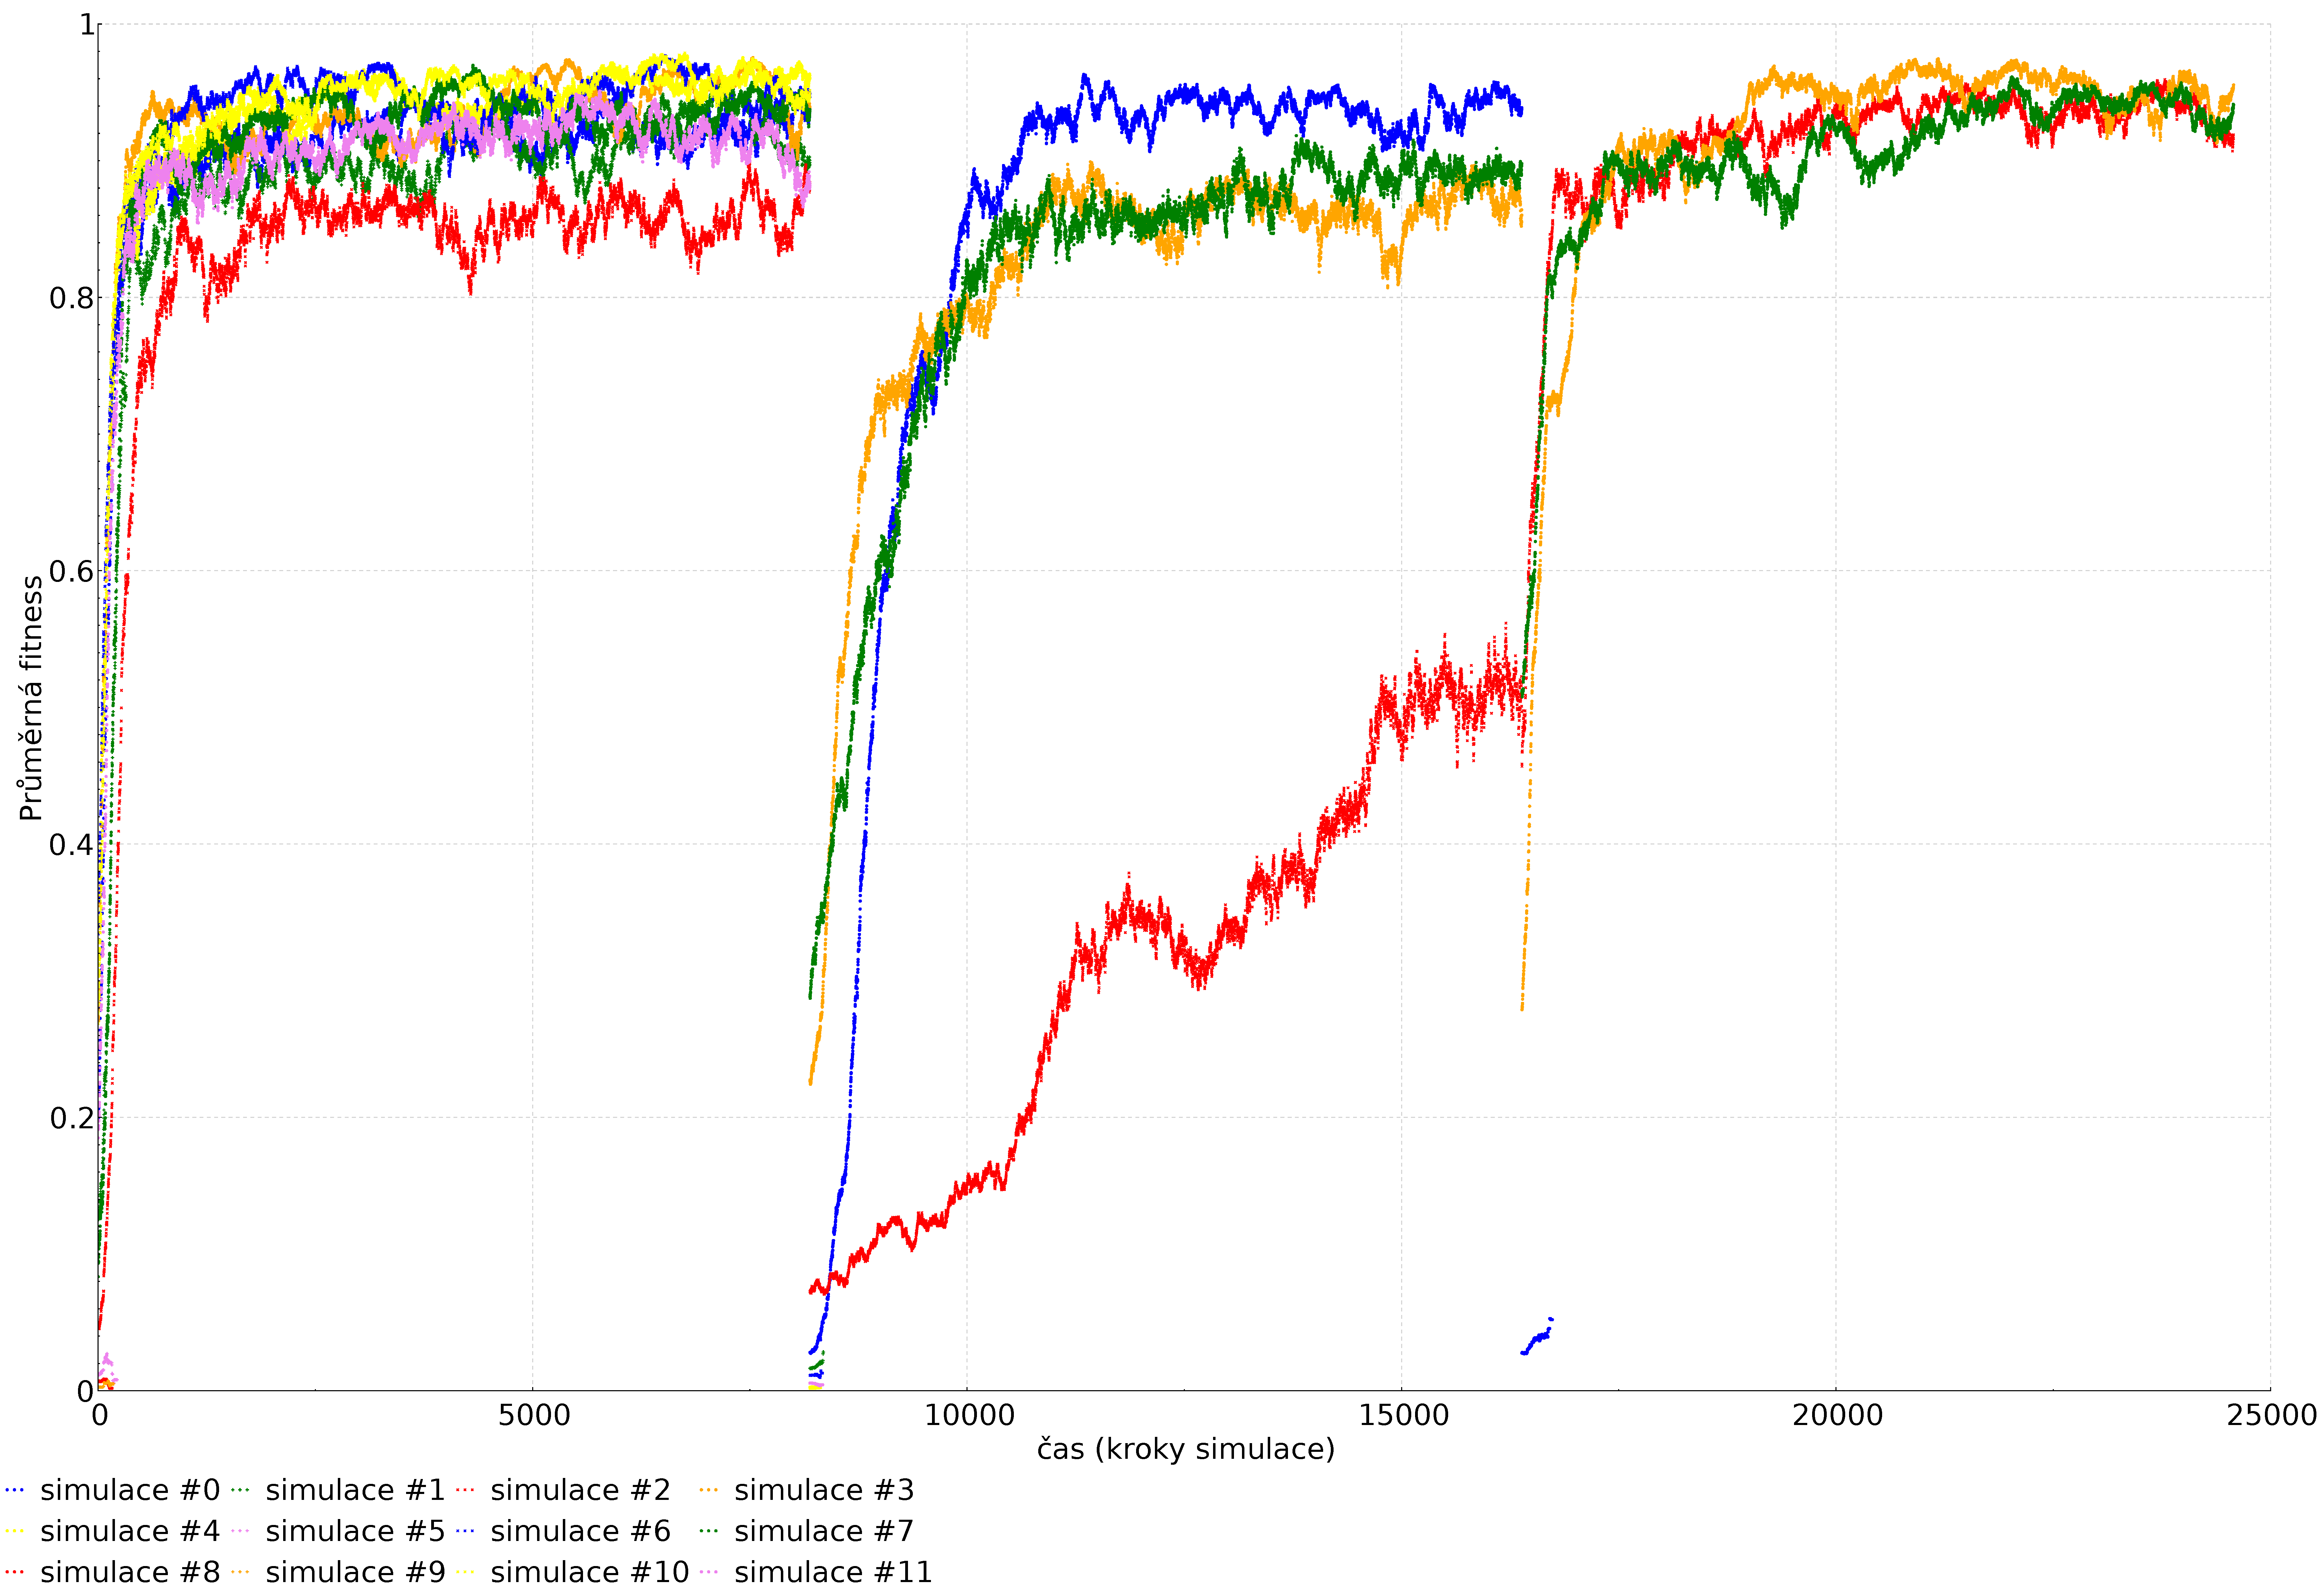
\includegraphics[width=\textwidth]{img/avg_fitness_256_00_00.pdf}

\label{fig:avg_fitness_256_0.0_0.0}

\textit{Podíl alel s negativní dominancí je pravděpodobnost, že nově vzniklá alela bude ovlivňovat fenotyp v opačných
        směrech, pokud bude v lokusu jednou nebo dvakrát. Podíl pleiotropických alel je pravděpodobnost, že nově vzniklá alela
        bude ovlivňovat více složek fenotypu. Rovnovážná velikost populace byla 256 jedinců.}

\end{figure}


\begin{figure}[h]
\caption{Graf vývojů průměrně fitness dvanácti populací pro podíl pleiotropních alel 0.0 a pro podíl negativně
         dominantních alel 0.0}
\centering
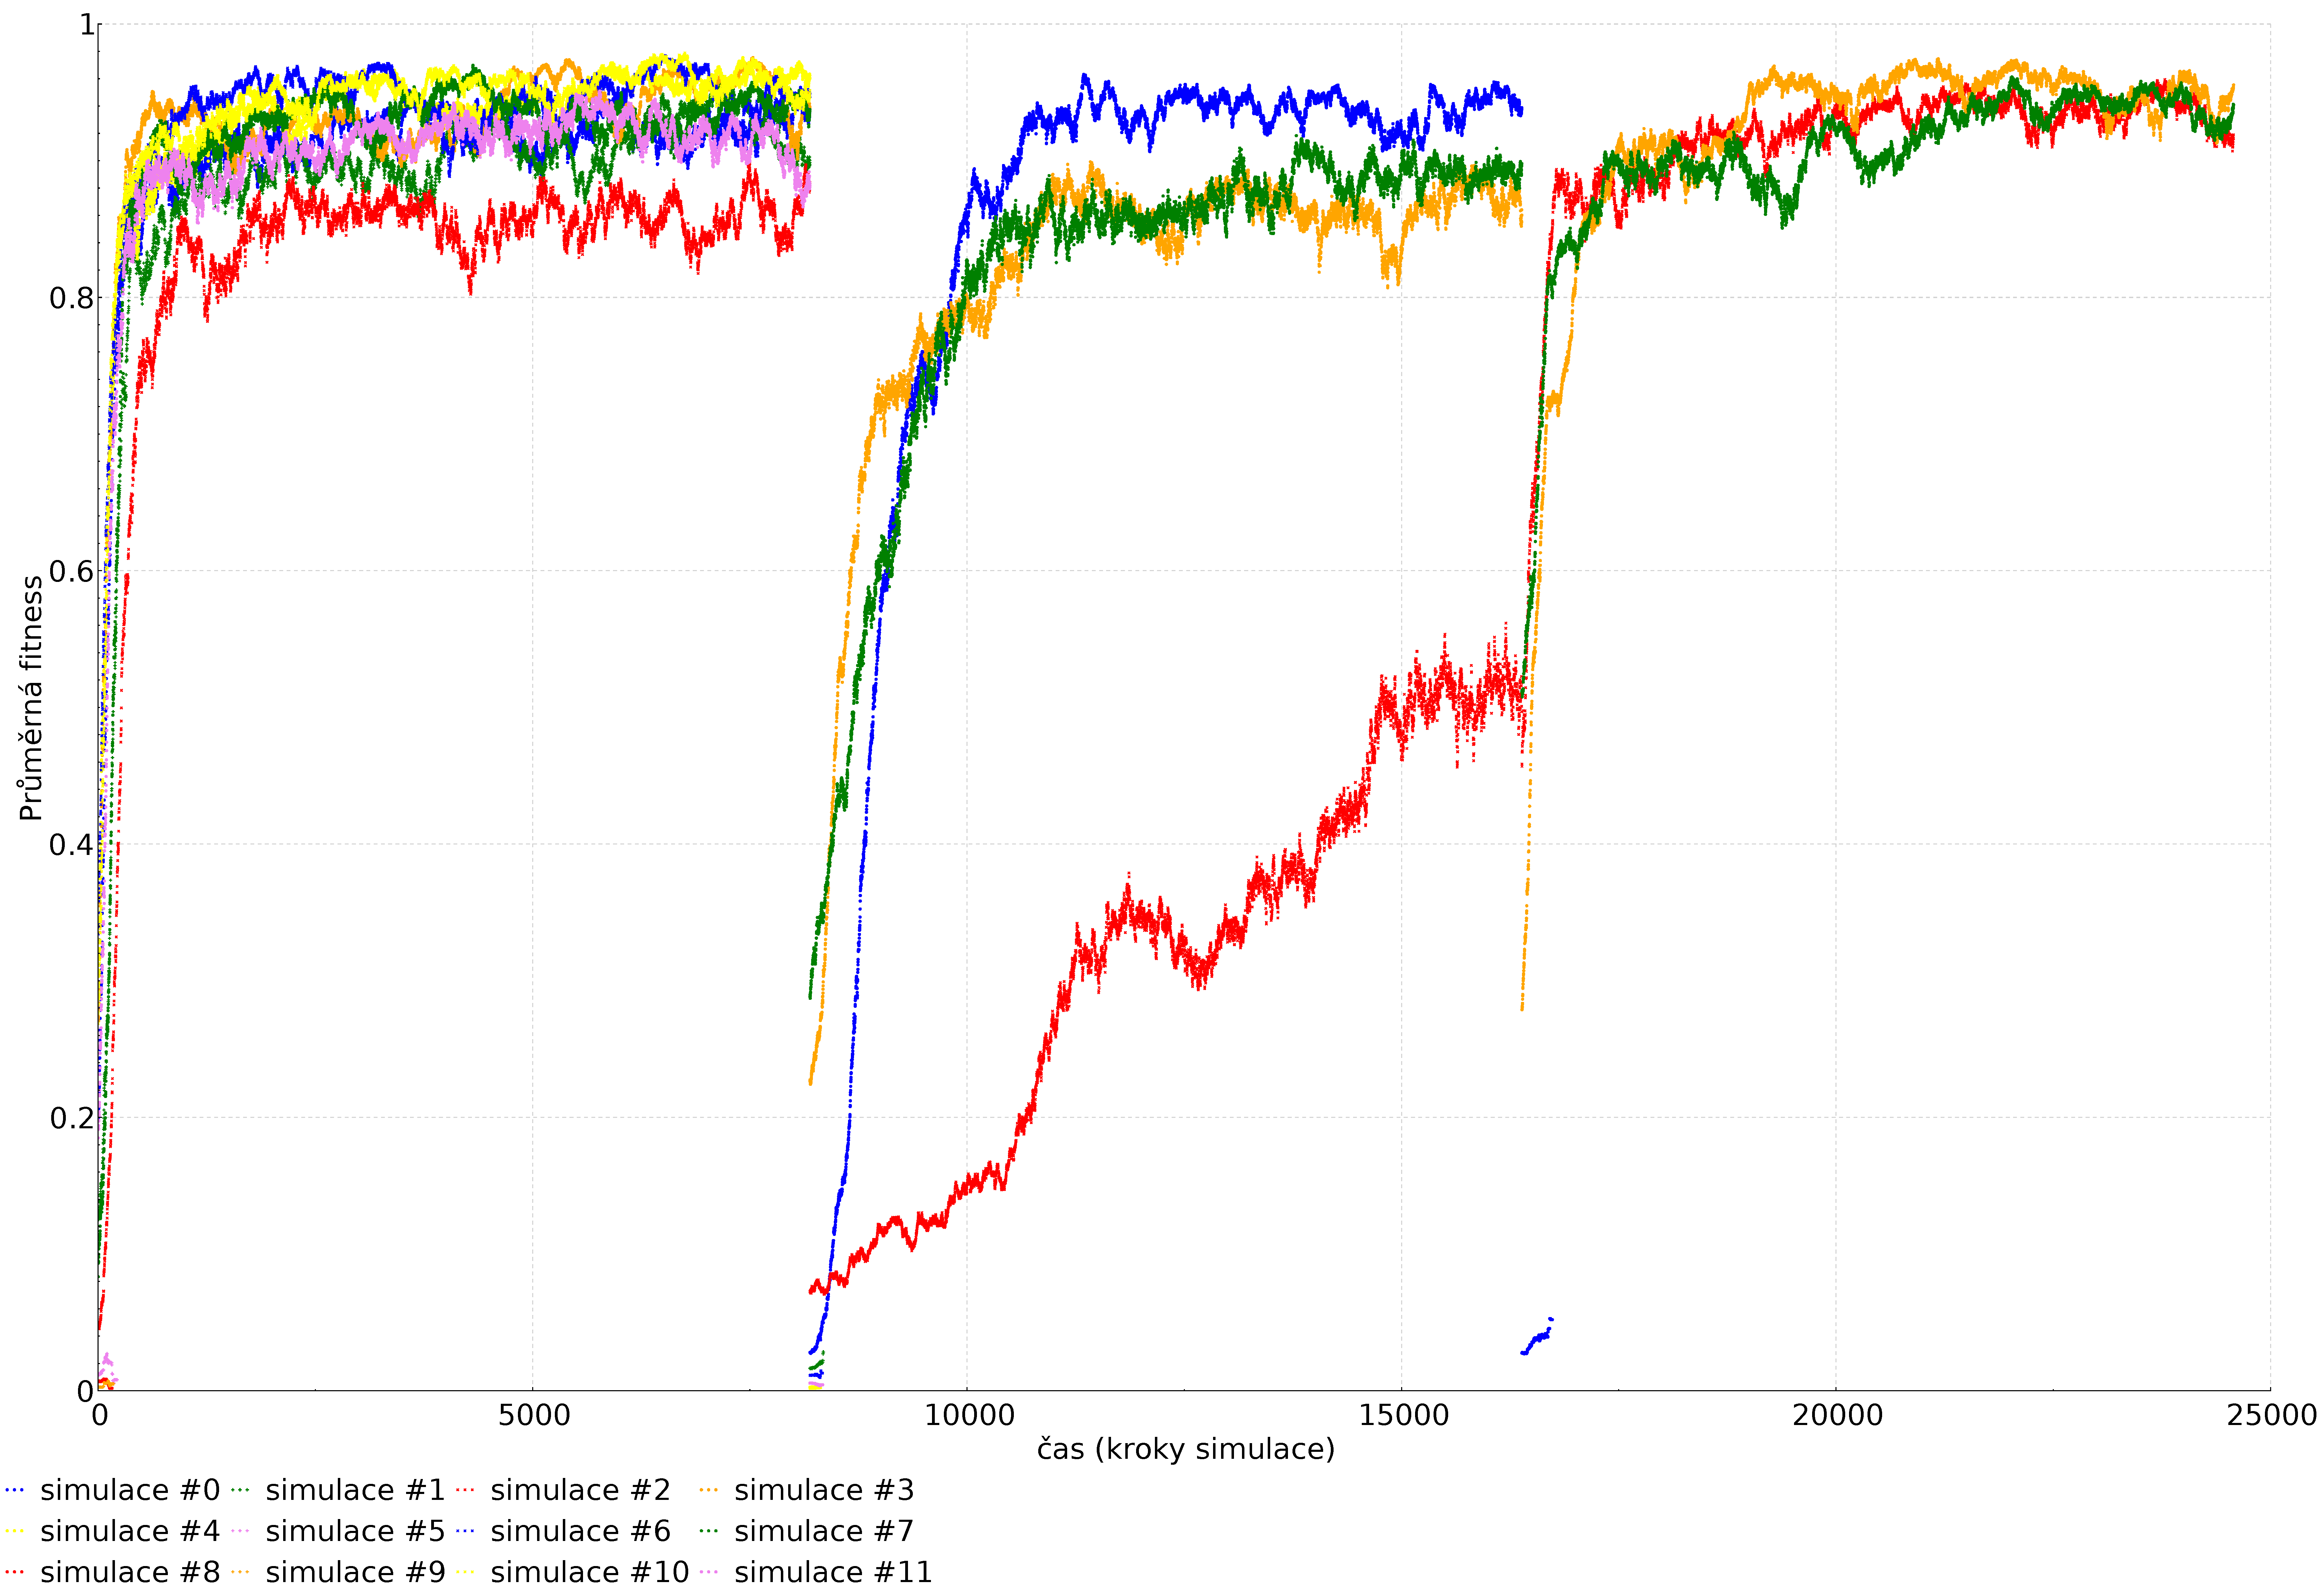
\includegraphics[width=\textwidth]{img/avg_fitness_256_00_00.pdf}

\label{fig:avg_fitness_sssssss256_0.0_0.0}

\textit{Legenda viz legenda k obrázku \ref{fig:avg_fitness_256_0.0_0.0}}

\end{figure}

\begin{figure}[h]
\caption{Graf vývojů průměrně fitness dvanácti populací pro podíl pleiotropních alel 0.0 a pro podíl negativně
         dominantních alel 0.0}
\centering
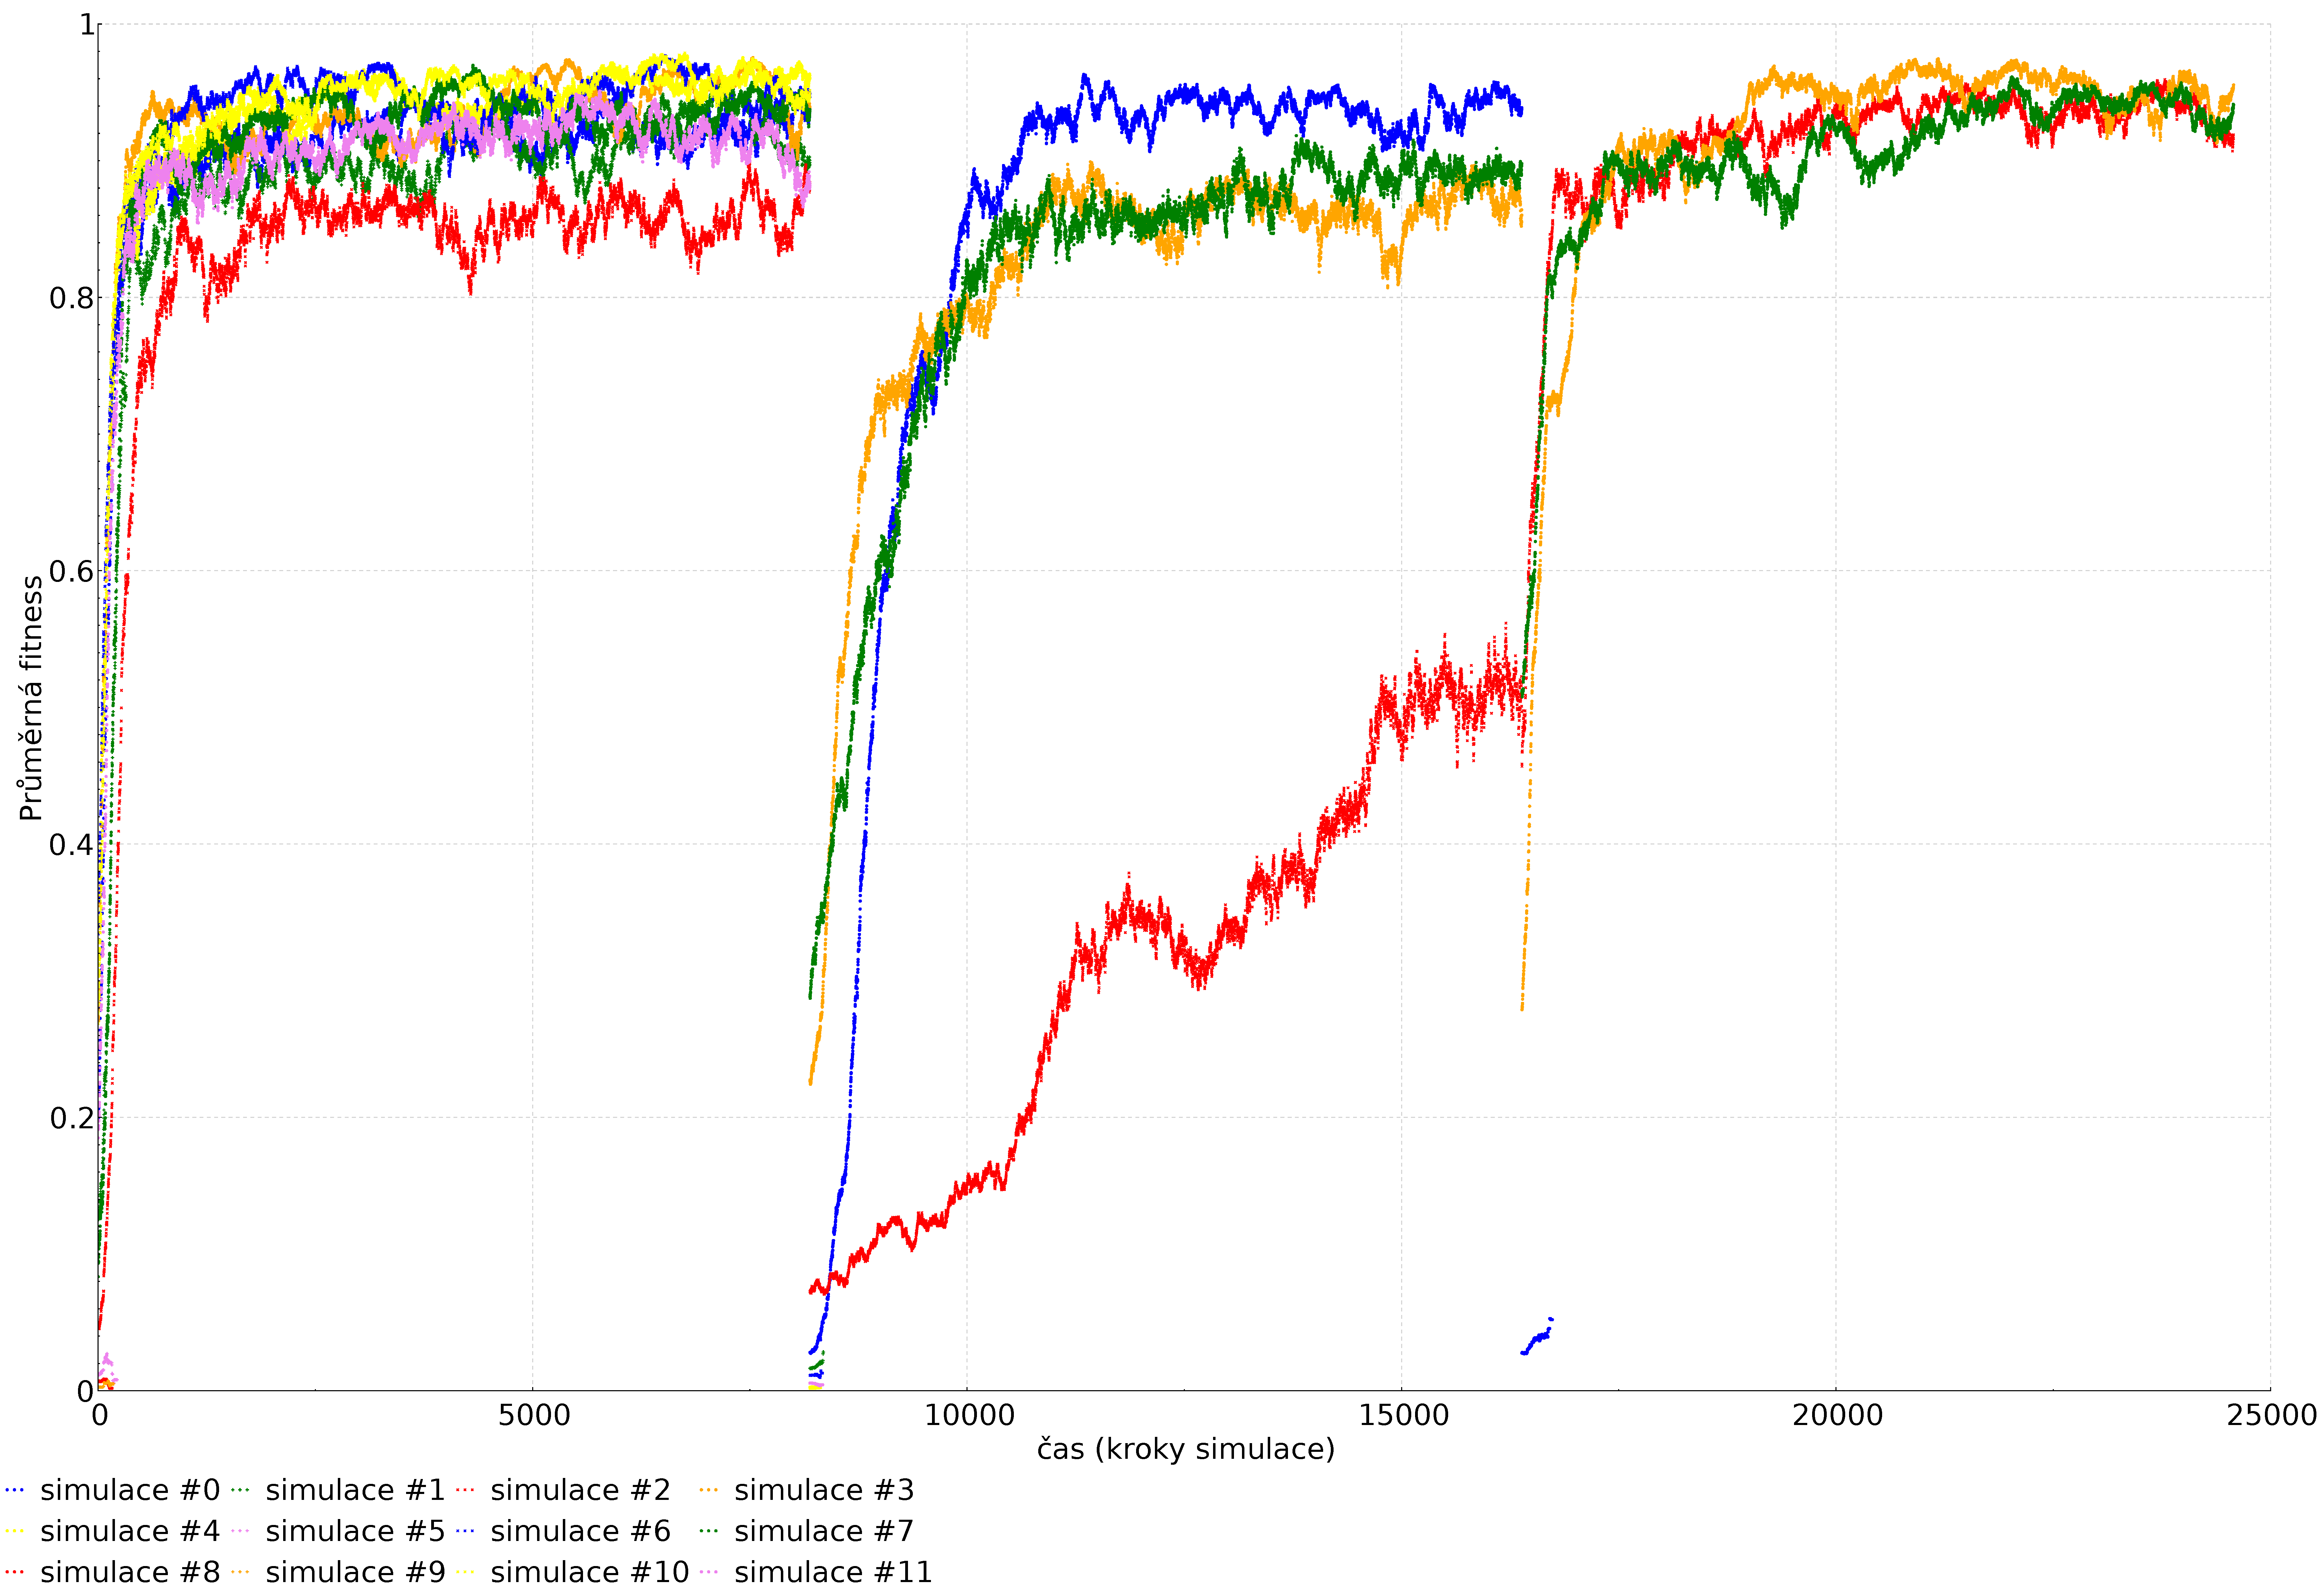
\includegraphics[width=\textwidth]{img/avg_fitness_256_00_00.pdf}

\label{fig:avg_fitness_2sss56_0.0_0.0}

\textit{Legenda viz legenda k obrázku \ref{fig:avg_fitness_256_0.0_0.0}}

\end{figure}

\openright
\end{document}
